\chapter{CR power plant simulation}
\section{Design  and simulation} \label{CR power plant design  and simulation}
%For the CR power plant simulation in SAM the “CSP power tower molten salt" model was used. The EPW weather file for Upington from Section~\ref{Location and weather data} was used as an input file to specify the hourly atmospheric conditions. SAM uses the following input data for the simulation:
For the CR plant simulation in SAM, the \enquote{CSP power tower molten salt} model was used. The EPW weather file for Upington from Section~\ref{Solar radiation} was used as an input file to specify the hourly atmospheric conditions. SAM uses the following input data for the simulation:
\begin{itemize}
\item Latitude (\si{\degree})
\item Longitude (\si{\degree})
\item Elevation above sea level (\si{\metre})
\item DNI (\si{\watt\per\square\metre})
\item Atmospheric pressure (\si{\milli\bar})
\item Dry bulb temperature (\si{\celsius})
\item Wet bulb temperature (\si{\celsius})
\item Relative humidity (\si{\percent})
\item Wind velocity (\si{\metre\per\second})
\end{itemize}
This Chapter describes in detail the crucial inputs of the CR power plant components, namely the power cycle, heliostat field, tower and receiver and thermal energy storage (TES).

As already mentioned, financial parameters and the LCOE are calculated separately in Microsoft Excel using a simplified method which is documented in Appendix~\ref{ChapterLCOE} on Page \pageref{ChapterLCOE}.

\subsubsection{Simulated configurations}
%The simulated configurations had the goal to reach 90~\% of the scheduled production curve by using variation of solar multiple and full load hours of TES. Also the simulated configurations covers a broad view on the technology possibilities. As already mentioned in Section~\ref{Large scale concentrated solar power (CSP) plants} is the SM the ratio of the receivers thermal output to the power cycles thermal input at design point. So a CR system with a SM of 1 has a receiver and a heliostat field which provides the thermal power needed for the power block to run at full load at the system design point. A receiver and collector field with a SM of 1 don't produce enough thermal power to store energy in a TES while feeding the turbine. A CR system with a SM of 1 is just suitable for systems without TES. To covering the scheduled load the solar multiple was varied from 2 to 3.5 in steps of 0.5. Also the storage full load hours were varied from 8 to \SI{16}{h} in steps of \SI{2}{h}. The target of \SI{100}{MW} net capacity was reached with a gross capacity of \SI{111}{MW} with an estimated gross-to-net conversion factor of 0.90. Table~\ref{tbl: CR_OverallConfig} summarizes the simulated configurations.
The simulated configurations were to meet 90~\% of the scheduled production curve by using variation of solar multiples and full load hours of TES. As mentioned in Section~\ref{Large scale concentrated solar power (CSP) plants} the solar multiple (SM) is the ratio of the receiver's thermal output to the power cycles thermal input at the design point. Thus, a CR system with a SM of 1 has a receiver and a heliostat field which provides the thermal power needed for the power block to run at full load at the system design point. A receiver and collector field with an SM of 1 do not produce enough thermal power to store energy in a TES while also feeding the turbine. A CR system with a SM of 1 is just sufficient for systems without TES. In order to cover the expected load, the solar multiple was varied from 2 to 3.5 in steps of 0.5, while storage full load hours were varied from 8 to \SI{16}{h} in steps of \SI{2}{h}. The target of \SI{100}{MW} net capacity was reached with a gross capacity of \SI{111}{MW} with an estimated gross-to-net conversion factor of \si{0.90}. Table~\ref{tbl: CR_OverallConfig} summarizes the simulated configurations.

\begin{table}[!h]  
  \centering
	\begin{tabular}{ p{4.0cm}  C{1.0cm} C{0.3cm} C{0.3cm} C{0.3cm} C{0.3cm} C{0.3cm} | C{0.3cm} C{0.3cm} C{0.3cm} C{0.3cm} C{0.3cm} } 
	\hline	
\textbf{Item} & \textbf{Unit} & \multicolumn{10}{c}{\textbf{Value}} \\ \hline \hline
Net turbine capacity & \si{\mega\wattel} & \multicolumn{10}{c}{100} \\
Gross turbine capacity & \si{\mega\wattel} & \multicolumn{10}{c}{111} \\ \hline
Solar multiple & - & \multicolumn{5}{c}{2.0} & \multicolumn{5}{c}{2.5} \\
TES capacity & h &  8 & 10 & 12 & 14 & 16 &  8 & 10 & 12 & 14 & 16 \\ \hline 
Solar multiple & - & \multicolumn{5}{c}{3.0} & \multicolumn{5}{c}{3.5} \\
TES capacity & h &   8 & 10 & 12 & 14 & 16 &  8 & 10 & 12 & 14 & 16 \\ \hline 
\end{tabular}
\caption[Simulated CR solar multiple and thermal energy storage configurations.]{Simulated CR solar multiple and thermal energy storage  configurations.}\label{tbl: CR_OverallConfig}
\end{table}
\subsubsection{Power cycle}
The power cycle of the simulated CR system features a Rankine-cycle steam engine, two open feed-water heaters, a pre-heater, boiler and super-heater \cite{NREL2015a}. As mentioned above has the turbine a gross capacity of \SI{111}{\mega\wattel} and a nameplate (net) capacity of 100 \si{\mega\wattel}. 
\begin{table}[!h]  
  \centering
	\begin{tabular}{  p{7.0cm}  C{2.0cm}  C{2.0cm} } 
	\hline	
\textbf{Item} & \textbf{Value} & \textbf{Unit} \\ \hline \hline
Turbine design capacity, gross  & 111 & \si{\mega\wattel} \\ 
Turbine design capacity, net & 100 & \si{\mega\wattel} \\ 
Boiler operating pressure & 125 & bar \\ 
Design inlet temperature & 288 & \si{\celsius} \\ 
Design outlet temperature & 566 & \si{\celsius} \\ 
Cycle conversion efficiency & 41.2 & \% \\ 
Steam generator design thermal power & 269.42 & \si{\mega\wattth}  \\
Power block start-up time & 0.5 & h \\ 
Minimum required start-up temperature & 500 & \si{\celsius} \\
Plant availability  & 96 & \\
Condenser type & air-cooled & - \\ 
\hline
\end{tabular}
\caption[CR power block and condecer input parameter in SAM.]{CR power block and condecer input parameter in SAM.}\label{tbl: CRPowerplant}
\end{table}
The steam generator has a HTF inlet temperature of \SI{566}{\celsius} and outlet temperature of \SI{288}{\celsius} at design point and operates at a pressure of \SI{125}{\bar}. In combination with a air-cooled condenser the CR power cycle system was simulated with a cycle gross efficiency of \SI{41.2}{\percent}. A wet-cooled condenser would reaches some higher efficiency, but because of the lack of water in the area of Upington and the requirement by the South African government for CSP plants, a air-cooled condenser was selected. The HTF inlet temperature, pressure and efficiency values where adapted for the configuration from \cite{Kolb2011a}. For starting up the system 
needs 30 minutes and a min. required temperature of \SI{500}{\celsius}. A plant availability of 96~\% was adapted from \cite{Morin2012} in order to simulate system down-times for outages or scheduled maintenance.
\subsubsection{Heliostat field}
The heliostat field design was done in SAM using its heliostat field layout optimization tool. For the design, optimization and simulation process, heliostat data from the Sanlúcar 120 heliostat was used \cite{Noone2012}. The Sanlúcar 120 is used in the Planta Solar 10 (PS10) near Seville, Spain and is the origin of Abengoas actual heliostat ASUP 140. For a simulation with the ASUP 140 no sufficient data was available. 
\begin{table}[!htbp]  
  \centering
	\begin{tabular}{ p{4.5cm}  C{1.5cm} C{1.2cm} C{1.2cm} C{1.2cm} C{1.2cm} } 
	\hline	
\textbf{Item} & \textbf{Unit} & \multicolumn{4}{c}{\textbf{Value}} \\ \hline \hline
racking & - &  \multicolumn{4}{c}{two-axis} \\
Height & m  &  \multicolumn{4}{c}{9.45} \\
Width & m  &  \multicolumn{4}{c}{12.84} \\
Reflective area & \si{\square\metre} &  \multicolumn{4}{c}{120.00} \\
Heliostat availability& \% &  \multicolumn{4}{c}{99} \\
Design-point DNI & \si{\watt\per\square\metre} &  \multicolumn{4}{c}{950} \\
\hline
\textbf{Solar multiple}& \textbf{-} & \textbf{2.0} & \textbf{2.5} & \textbf{3.0} & \textbf{3.5}\\ \hline 
Number of heliostats & - & 9~131 & 11~530 & 13~976 & 16~658 \\
Max. distance from tower & m & 1~528 & 1~708 & 1~883 & 2010 \\
Reflective area  & ha & 109.58 & 138.36 & 167.72 & 199.90 \\
Field land area & ha & 655.59 & 821.92 & 997.95 & 1~190.99 \\ 
\hline
\end{tabular}
\caption[CR heliostat parameter.]{CR heliostat parameter.}\label{tbl: CRHeliostats}
\end{table}
The Sanlúcar 120 heliostats have an effective reflective area of \SI{120}{\square\metre} and are tracked on 2 axes. The heliostat field layout optimization and there design depends on the turbine gross and the SM. The heliostat field was optimized therefore for all four considered configurations. SAM first generates a coarse layout and optimizes the number of heliostats and their position. The goal of the optimization is the maximum flux with minimum power constraints according to the specified design-point DNI which represents the DNI at which the power plant achieves its rated thermal capacity. Table~\ref{tbl: CRHeliostats} summarizes the heliostat datas and the values of the optimized field design for all considered solar multiples.

The optimized heliostat field layouts of the four considered SM are depict in Figure~\ref{SM}. In order to avoid mutual shading from the heliostats the heliostat density decreases with distance from the tower. The maximum heliostat distance to the tower rises with the higher SM which can be seen in the field diameter. 
\begin{figure}[!htbp]
        \centering   
        \begin{subfigure}[b]{0.5\textwidth}
                \centering
                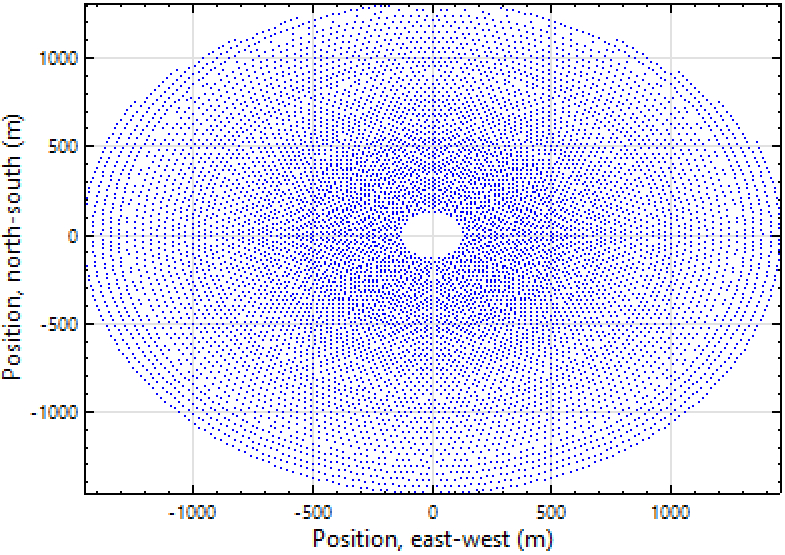
\includegraphics[width=0.95\textwidth]{FIG/SM20}
                \caption{SM:~2.0}\label{SM2.0}
        \end{subfigure}%
        ~
        \begin{subfigure}[b]{0.5\textwidth}
                \centering
                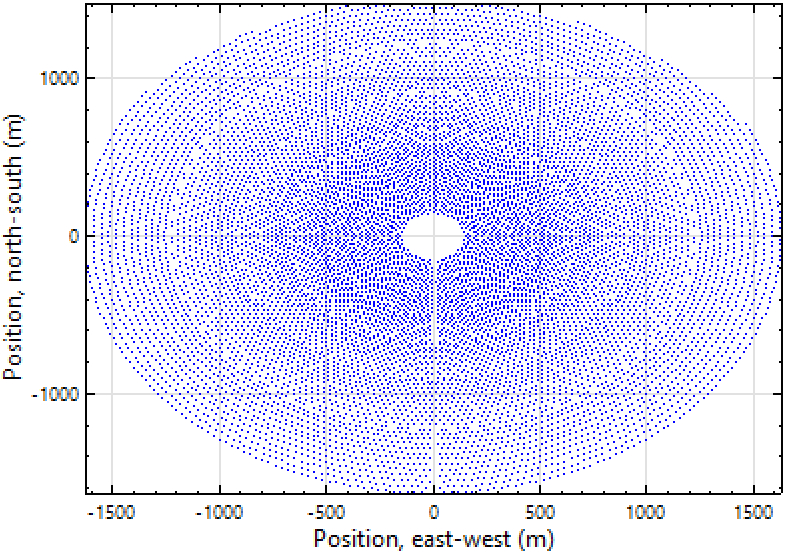
\includegraphics[width=0.95\textwidth]{FIG/SM25}
                \caption{SM:~2.5}\label{SM2.5}
        \end{subfigure}
        
\par\medskip % Linebreak
                
        \begin{subfigure}[b]{0.5\textwidth}
                \centering
                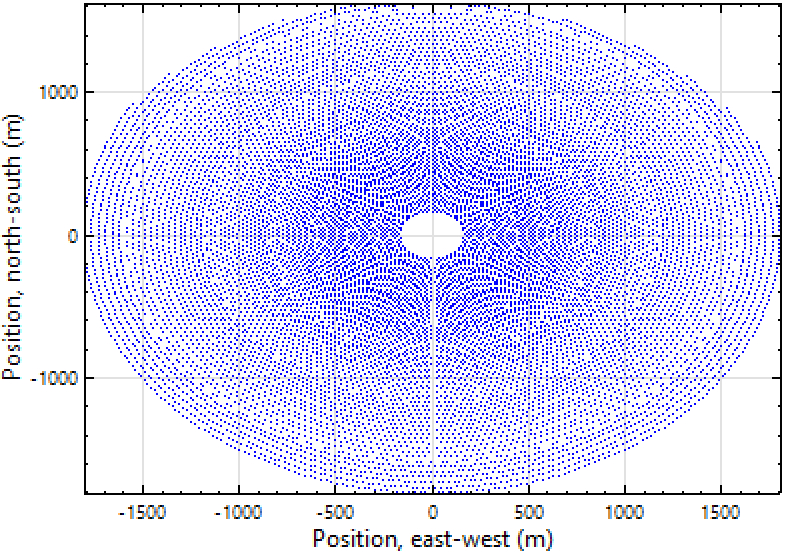
\includegraphics[width=0.95\textwidth]{FIG/SM30}
                \caption{SM:~3.0}\label{SM3.0}
        \end{subfigure}%
        ~
        \begin{subfigure}[b]{0.5\textwidth}
                \centering
                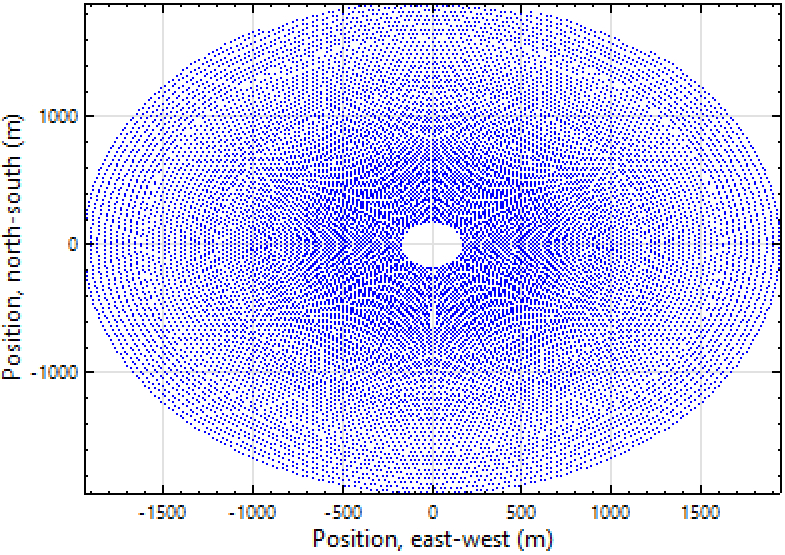
\includegraphics[width=0.95\textwidth]{FIG/SM35}
                \caption{SM:~3.5}\label{SM3.5}
        \end{subfigure}
        \caption[Simulated heliostat field layout at diferent solar multiples (SM).]{Simulated heliostat field layout at diferent solar multiples (SM).}\label{SM}
\end{figure}
\subsubsection{Tower and receiver}
The receiver collects the concentrated irradiance from the surrounding heliostat field. The simulated receiver is build as an external cylindrical receiver and is configurated with 24 panels of thin walled (1.25 mm) receiver tubes with an outer diameter of 60 mm arranged in a circle around the tower. The receiver tubes are made from 316H stainless steel and the external surfaces of the tubes are coated with a black Pyromark paint. The paint is resistant to high temperatures and thermal cycling, and absorbed 95\% of the incident sunlight. This configuration is similar to the receiver of the  Solar Two Project accept of the outer diameter \cite{Bradshaw2002}. The panels containing molten salt (60~\% NaNO\textsubscript{3} and 40~\% KNO\textsubscript{3}) as heat transfer fluid (HTF). The receiver design inlet temperature of 288$\,^{\circ}\mathrm{C}$ and the outlet temperature of 566$\,^{\circ}\mathrm{C}$ was set before in the power block configuration. In order to achieve the desired receiver thermal power output, the height of the tower and receiver dimensions got also adjust with the optimization of the heliostat field design. The results of the optimization is shown in Table~\ref{tbl: CRSolarfield}, as well as the fixed tower and receiver parameter. The heights of the tower range from 179.77 to \SI{236.50}{m}. The receiver proportions rises with the SM and the field sizes and results in a receiver thermal power range from 538.8 to 943.0 \si{\mega\wattth}.
\begin{table}[!h]  
  \centering
	\begin{tabular}{ p{5.5cm}  C{1.5cm} C{1.2cm} C{1.4cm} C{1.4cm} C{1.4cm} } 
	\hline	
\textbf{Item} & \textbf{Unit} & \multicolumn{4}{c}{\textbf{Value}} \\ \hline \hline
Receiver configuration & - &  \multicolumn{4}{c}{external cylindrical receiver}\\
Heat transfer fluid & - &  \multicolumn{4}{c}{60~\% NaNO\textsubscript{3} and 40~\% KNO\textsubscript{3}}\\
Inlet temperatures & $\,^{\circ}\mathrm{C}$  &  \multicolumn{4}{c}{288}\\
Outlet temperatures & $\,^{\circ}\mathrm{C}$  &  \multicolumn{4}{c}{566}\\
Receiver tube material & - &  \multicolumn{4}{c}{AISI316 stainless steal}\\
Receiver tube outer diameter & \si{\milli\metre} &  \multicolumn{4}{c}{60}\\
Receiver tube wall thickness & \si{\milli\metre} &  \multicolumn{4}{c}{1.25}\\
Number of panels & - &  \multicolumn{4}{c}{24}\\
Absorption factor  & - &  \multicolumn{4}{c}{0.95}\\
\hline
\textbf{Solar multiple} &  & \textbf{2.0} & \textbf{2.5} & \textbf{3.0} & \textbf{3.5}\\ \hline 
Tower height & \si{\metre} & 179.77 & 200.96 & 221.57 &  236.50\\
Receiver height  & \si{\metre} & 22.55 & 25.45 & 27.74 &  29.94\\
Receiver diameter & \si{\metre} & 14.85 & 16.66 & 17.91 & 18.77\\ 
Receiver aperture area & \si{\square\metre} & 1~052 & 1~332 & 1~561 & 1~765 \\ 
Receiver thermal power & \si{\mega\wattth} & 538.8 & 673.5 & 808.3 & 943.0 \\
\hline
\end{tabular}
\caption[CR heliostat field parameter.]{CR heliostat field parameter.}\label{tbl: CRSolarfield}
\end{table}
\subsubsection{Thermal energy storage (TES)}
The CR system was simulated using a direct two-tank molten salt thermal energy storage (TES). The storage uses directly the HTF (60~\% NaNO\textsubscript{3} and 40~\% KNO\textsubscript{3}) from the receiver as storage medium. Figure~\ref{towerdirecttwotank} on Page~\pageref{towerdirecttwotank} shows a schema of the direct storage for CR system. The design temperature of the hot storage tank (566$\,^{\circ}\mathrm{C}$) and the cold storage tank (288$\,^{\circ}\mathrm{C}$) depends also from the set value in the power block settings as before the design receiver temperatures. So the design temperature difference between the tanks is 278$\,^{\circ}\mathrm{C}$.



As defined at the beginning of this Chapter, the full load hours of TES are varied in steps of \SI{2}{h} from 8 to \SI{16}{h}. The TES full load hours represents the time in which the storage can supply enough energy to the steam turbine and the power block to run at full design capacity. So a higher value of TES full load hours extended the time that the power plant can run during nights or cloudy days. Table~\ref{tbl: CRTES} shows that with higher TES full load hours the thermal capacity and tank volume increases as well. The simulated storage capacity is in a range of 2~\SI{155}{\mega\wattth\hour} using 8 full load hours and 4~\SI{311}{\mega\wattth\hour} using 16 full load hours. 
\begin{table}[!h]  
  \centering
	\begin{tabular}{ p{3.9cm}  C{1.0cm} C{1.2cm} C{1.2cm} C{1.2cm} C{1.2cm} C{1.2cm} } 
	\hline	
\textbf{Item} & \textbf{Unit} & \multicolumn{5}{c}{\textbf{Value}} \\ \hline \hline
Storage type & - &  \multicolumn{5}{c}{direct two-tank molten salt}\\
Storage fluid & - &  \multicolumn{5}{c}{60~\% NaNO\textsubscript{3} and 40~\% KNO\textsubscript{3}}\\
Hot tank design temp. & \si{\celsius} & \multicolumn{5}{c}{566}\\
Cold tank design temp. & \si{\celsius} & \multicolumn{5}{c}{288}\\
\hline
\textbf{TES full load hours} & \textbf{h} & \textbf{8} & \textbf{10} & \textbf{12} & \textbf{14} & \textbf{16}\\ \hline 
Thermal capacity & \si{\mega\wattth\hour} & 2~155 & 2~694 & 3~233 & 3~772 &  4~311\\
Storage volume  & \si{\cubed\metre} & 10~229 & 12~787 & 15~345 & 17~902 & 20~460\\
\hline
\end{tabular}
\caption[CR system TES parameter.]{CR system TES parameter.}\label{tbl: CRTES}
\end{table}

SAM 2015.6.30 r3 don't have a power control to follow prescribed hourly net output values. The turbine output of each day needs to be scheduled in front for the simulation. Thereby the parasitic consumer needs highly attention. Figure~\ref{CR_turbineoutput} shows the for the simulation scheduled turbine output matrix. The individual values was fixed during experimental trial. It can be seen that the turbine output is reduced to 50\% during the night as it is specified in the scenario. The power plant follows the schedule till there is no solar irradiance and no more thermal capacity in the storage left to generate power. 
\begin{figure}[htbp]  
\centering
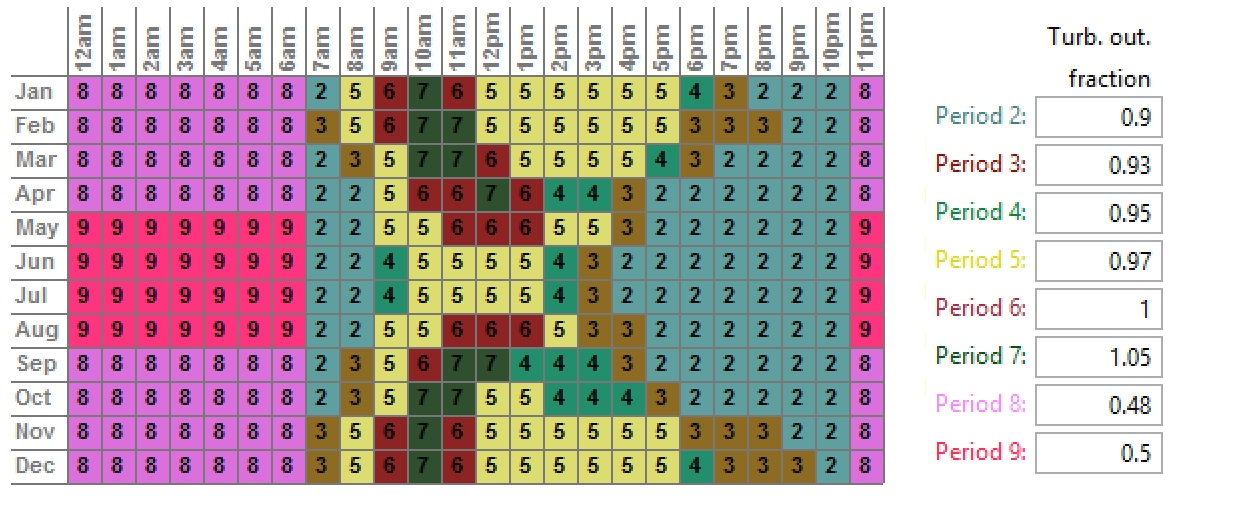
\includegraphics[width=0.95\linewidth]{FIG/CR_turbineoutput}
\caption[TES dispatch control matrix for turbine output fraction of CR simulation in SAM.]{TES dispatch control matrix for turbine output fraction of CR simulation in SAM.}\label{CR_turbineoutput}
\end{figure}
\pagebreak
\subsubsection{Financial parameter}
The financial parameter for the LCOE calculation of the CR power plant are seperated in different specific cost parts and are sumerized in Table~\ref{tbl: CRFinance}. The method for calculating the LCOE is documented in Appendix~\ref{ChapterLCOE} on Page \pageref{ChapterLCOE} using a lifetime of \SI{25}{years} and a real interest rate of 7.5~\% \cite{FraunhoferISE2013}. The interest rate could be reduced with a rising market potential.




The specific costs of the heliostat field of \SI{180}{\usd\per\square\metre} coming from J. B. Blackmon \cite{Blackmon2012}. He analyzed the costs of heliostat as a function of area for a representative solar central receiver power plant and calculated the total installed costs for a field of 5~000 heliostats with \SI{148}{\square\metre} reflective area of approximately \SI{180}{\usd\per\square\metre}. The analyze results showed that the costs are increasing with the size of the heliostats from \SI{40}{\square\metre} on. So the adopted value of \SI{180}{\usd\per\square\metre} reflective area for \SI{140}{\square\metre} heliostats can be assumed as conservative.


The remaining investment costs are based on the "Power Tower Technology Roadmap and Cost Reduction Plan" \cite{Kolb2011} from 2011.

On top of the investment costs a came 15 \% once-off surcharge for EPC and contingencies \cite{Platzer2014}.

Fichtner analyzed the annual O\&M costs with 1.84-1.96~\% of the total investment costs for CR power plants in SA \cite{Fichtner2010}. The value of 2~\% can so also be assumed as conservative.

The costs for the land purchase comes from the "African Agriculture Review" report of the Nedbank Capital, which reported the prices for farmland in SA. For the LCOE calculation of the CSP and PV system was the land purchase costs of 3~\SI{000}{USD/ha} assumed which is based on these report \cite{Cassell2012}.

\begin{table}[!h]  
  \centering
	\begin{tabular}{  p{5.0cm} C{2.0cm} C{1.5cm}  C{1.5cm}  C{4.0cm} } 
	\hline	
\textbf{Item} & \textbf{Symbol}& \textbf{Value} & \textbf{Unit} & \textbf{Source}\\ \hline \hline
Heliostat field &$c_{HF}$ & 180 & \si{\usd\square\metre} & \cite{Blackmon2012}\\ 
Power block & $c_{PB,CR}$ & 1000 & \si{\usd\per\kilo\wattel} & \cite{Kolb2011}\\ 
Thermal energy storage&$c_{TES,CR}$ & 30 & \si{\usd\per\kilo\wattth\hour}  & \cite{Kolb2011}\\ 
Tower and receiver& $c_{T+R}$& 200 & \si{\usd\per\kilo\wattth} & \cite{Kolb2011}\\ 
Annual O\&M & $f_{O\&M,CR}$ & 2 & \si{\percent} &\cite{Fichtner2010}\\
Land purchase& $c_{LP}$ & 3~000 & \si{\usd\per\hectare} & \cite{Cassell2012}\\ \hline
Lifetime & $n$ & 25 & years & \cite{FraunhoferISE2013} \\ 
Interest rate & $i_{CR}$ & 7.5 & \si{\percent} & \cite{FraunhoferISE2013} \\ 
Annual insurance costs& $f_{ins,CR}$ & 0.5 & \si{\percent} & \cite{IRENA2012}\\
Surcharge for EPC, project management and risk & $f_{EPC,CR}$& 15 & \si{\percent} & \cite{Platzer2014} \\
Total plant availability & $f_{avail,plant,CR}$ & 96 & \si{\percent} & \cite{Morin2012} \\ 
\hline
\end{tabular}
\caption[Finacial input parameter for CR-simulation in SAM.]{Finacial input parameter for CR-simulation in SAM.}\label{tbl: CRFinance}
\end{table}
\section{Results of CR power plant simulation}
The following sections illustrates and discuss the obtained simulation and calculation results of the above defined CR power plant. Therefore the load curve covering performance and LCOE as well as the belonging load profiles and duration curves are described and analyzed. The configuration of the power plants to reach 90~\% of the prescribed load while using the best belonging LCOE is defined at the end of each section.
\subsubsection{Load curve covering}
To find the suitable power plant configuration of the CR system to reach the target of 90~\% load curve covering, there was 20 various configurations simulated. This section presets and compare mainly the results of the simulation with the lowest SM and hours of TES configuration (SM: 2.0 \& TES: \SI{8}{h}) with the simulation using the highest SM and hours of TES configuration (SM: 3.5 \& TES: \SI{16}{h}) representative for all in between. All simulated configurations are shown in Table~\ref{tbl: CR_OverallConfig} on Page~\pageref{tbl: CR_OverallConfig}.

\begin{figure}[htbp]  
\centering
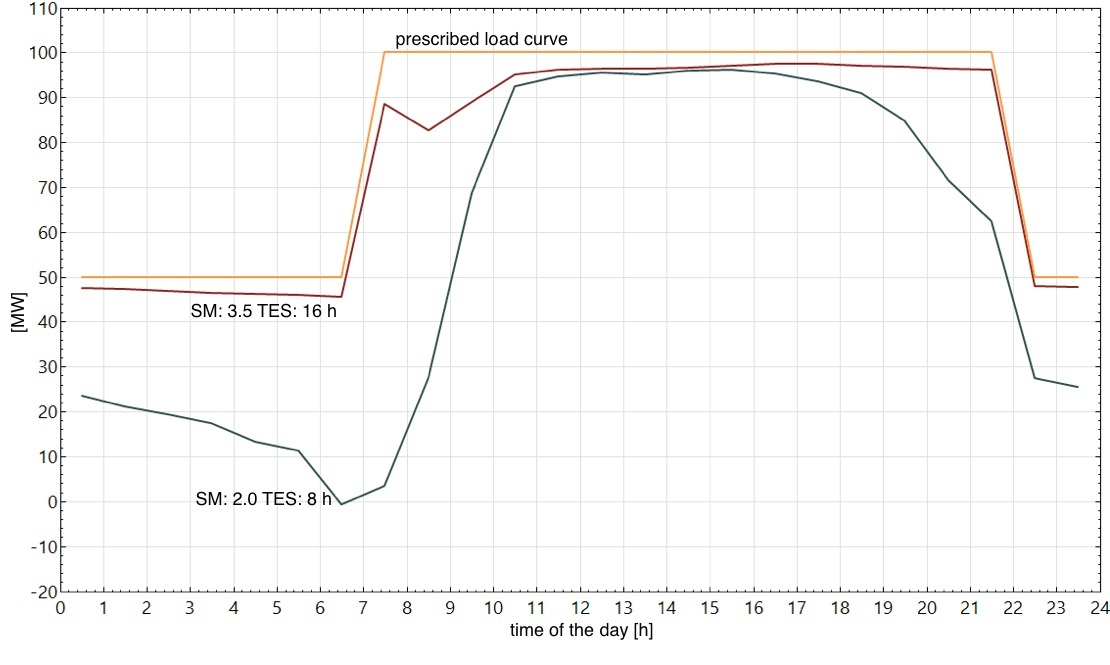
\includegraphics[width=0.8\linewidth]{FIG/CR_annual_profil}
\caption[Annual average load profile of selected CR power plant configurations.]{Annual average load profile of selected CR power plant configurations.}\label{CR_annual_profil}
\end{figure}
Figure~\ref{CR_annual_profil} shows the annual load curve covering of the above mentioned CR power plant high and low configurations with the prescribed load curve. The Figure shows, that the CR power plant using a SM of 3.5 and \SI{16}{h} of TES for the configuration can cover almost at any time of the year the prescribed load curve. The decreasing of the supplied electricity 8:00 leads from the winter duration and will be shown in the following. The lower CR power plant configuration can just cover between 11:00 and 17:00 almost the same amount electricity during the year than the high configuration. In the morning times between 6:00 and 7:00 the energy production is coming to standstill the whole year. The results of all annual average load profiles can be found in Appendix~\ref{all_load_profile}.

At this point it might be necessary to remind, that it is just the electricity used for the annual load covering as well as for the LCOE calculation which is actually supplied at the requested time step. So the electricity which is overproduced at any time of the year is not considered. This can also be seen in Figure~\ref{CR_winter_load}. 
\begin{figure}[htbp]  
\centering
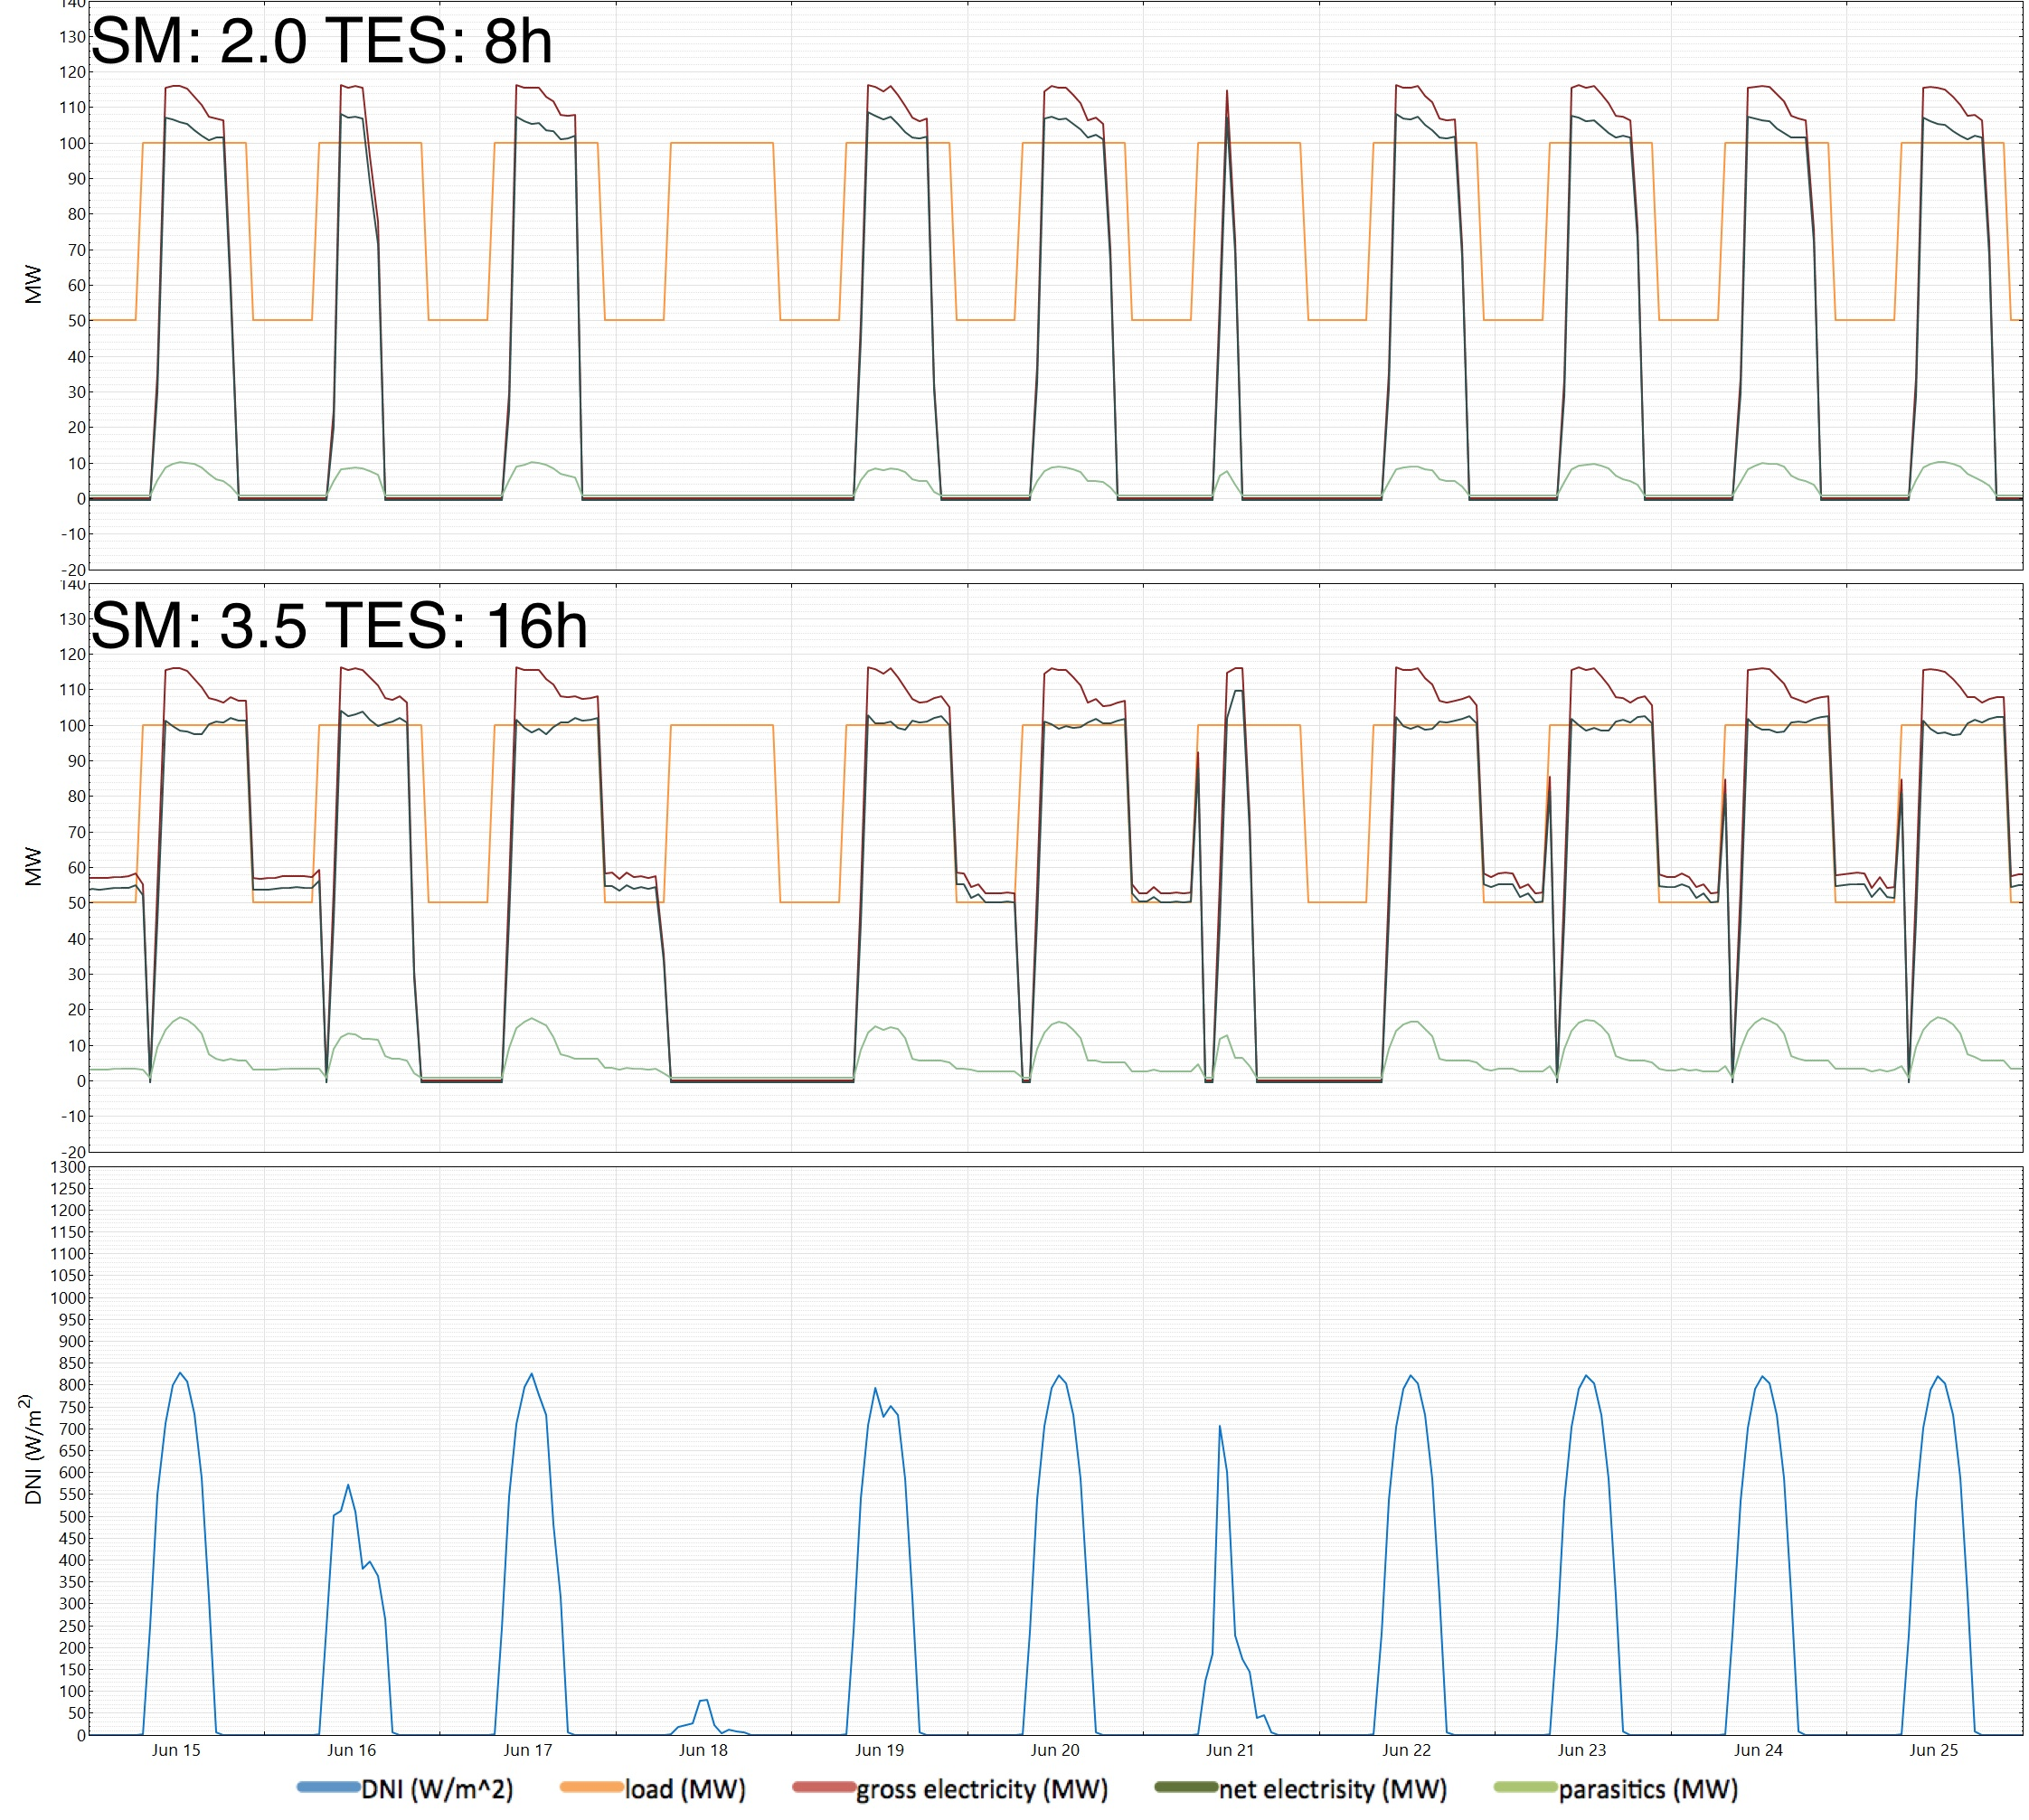
\includegraphics[width=1\linewidth]{FIG/CR_winter_load}
\caption[CR load profile during the time of winter solstice (15. June - 25. June).]{CR load profile during the time of winter solstice (15. June - 25. June).}\label{CR_winter_load}
\end{figure}
This figure shows exemplary the load curve behavior of the CR power plants during the time with the least hours of sunlight during a day of the year. The DNI is around \SI{830}{\watt\per\square\metre} in peak times at these days and there are also days with less or almost no direct irradiance. As mentioned, it can be seen that the net electricity production is in both cases at some times across the prescribed load curve and is not consulted further. This reaches mainly from the described dispatch control matrix from Figure~\ref{CR_turbineoutput} on Page~\pageref{CR_turbineoutput} to control the turbine output. This is not accurate at all to follow a specific load exactly during each day of the year. 

However, Figure~\ref{CR_winter_load} mainly shows the load curve behavior of the CR power plants in low and high configuration. At a SM of \si{2.0} with \SI{8}{h} of TES the power plant can't produce enough power during the day to fill up the TES for generating power during the night. Compared to that, the CR power plant with a SM of \si{3.5} and \SI{16}{h} of TES can almost anytime generate electricity over the whole night. But with the rising load in the morning hours the energy production stops due to the empty storage. 
\begin{figure}[htbp]  
\centering
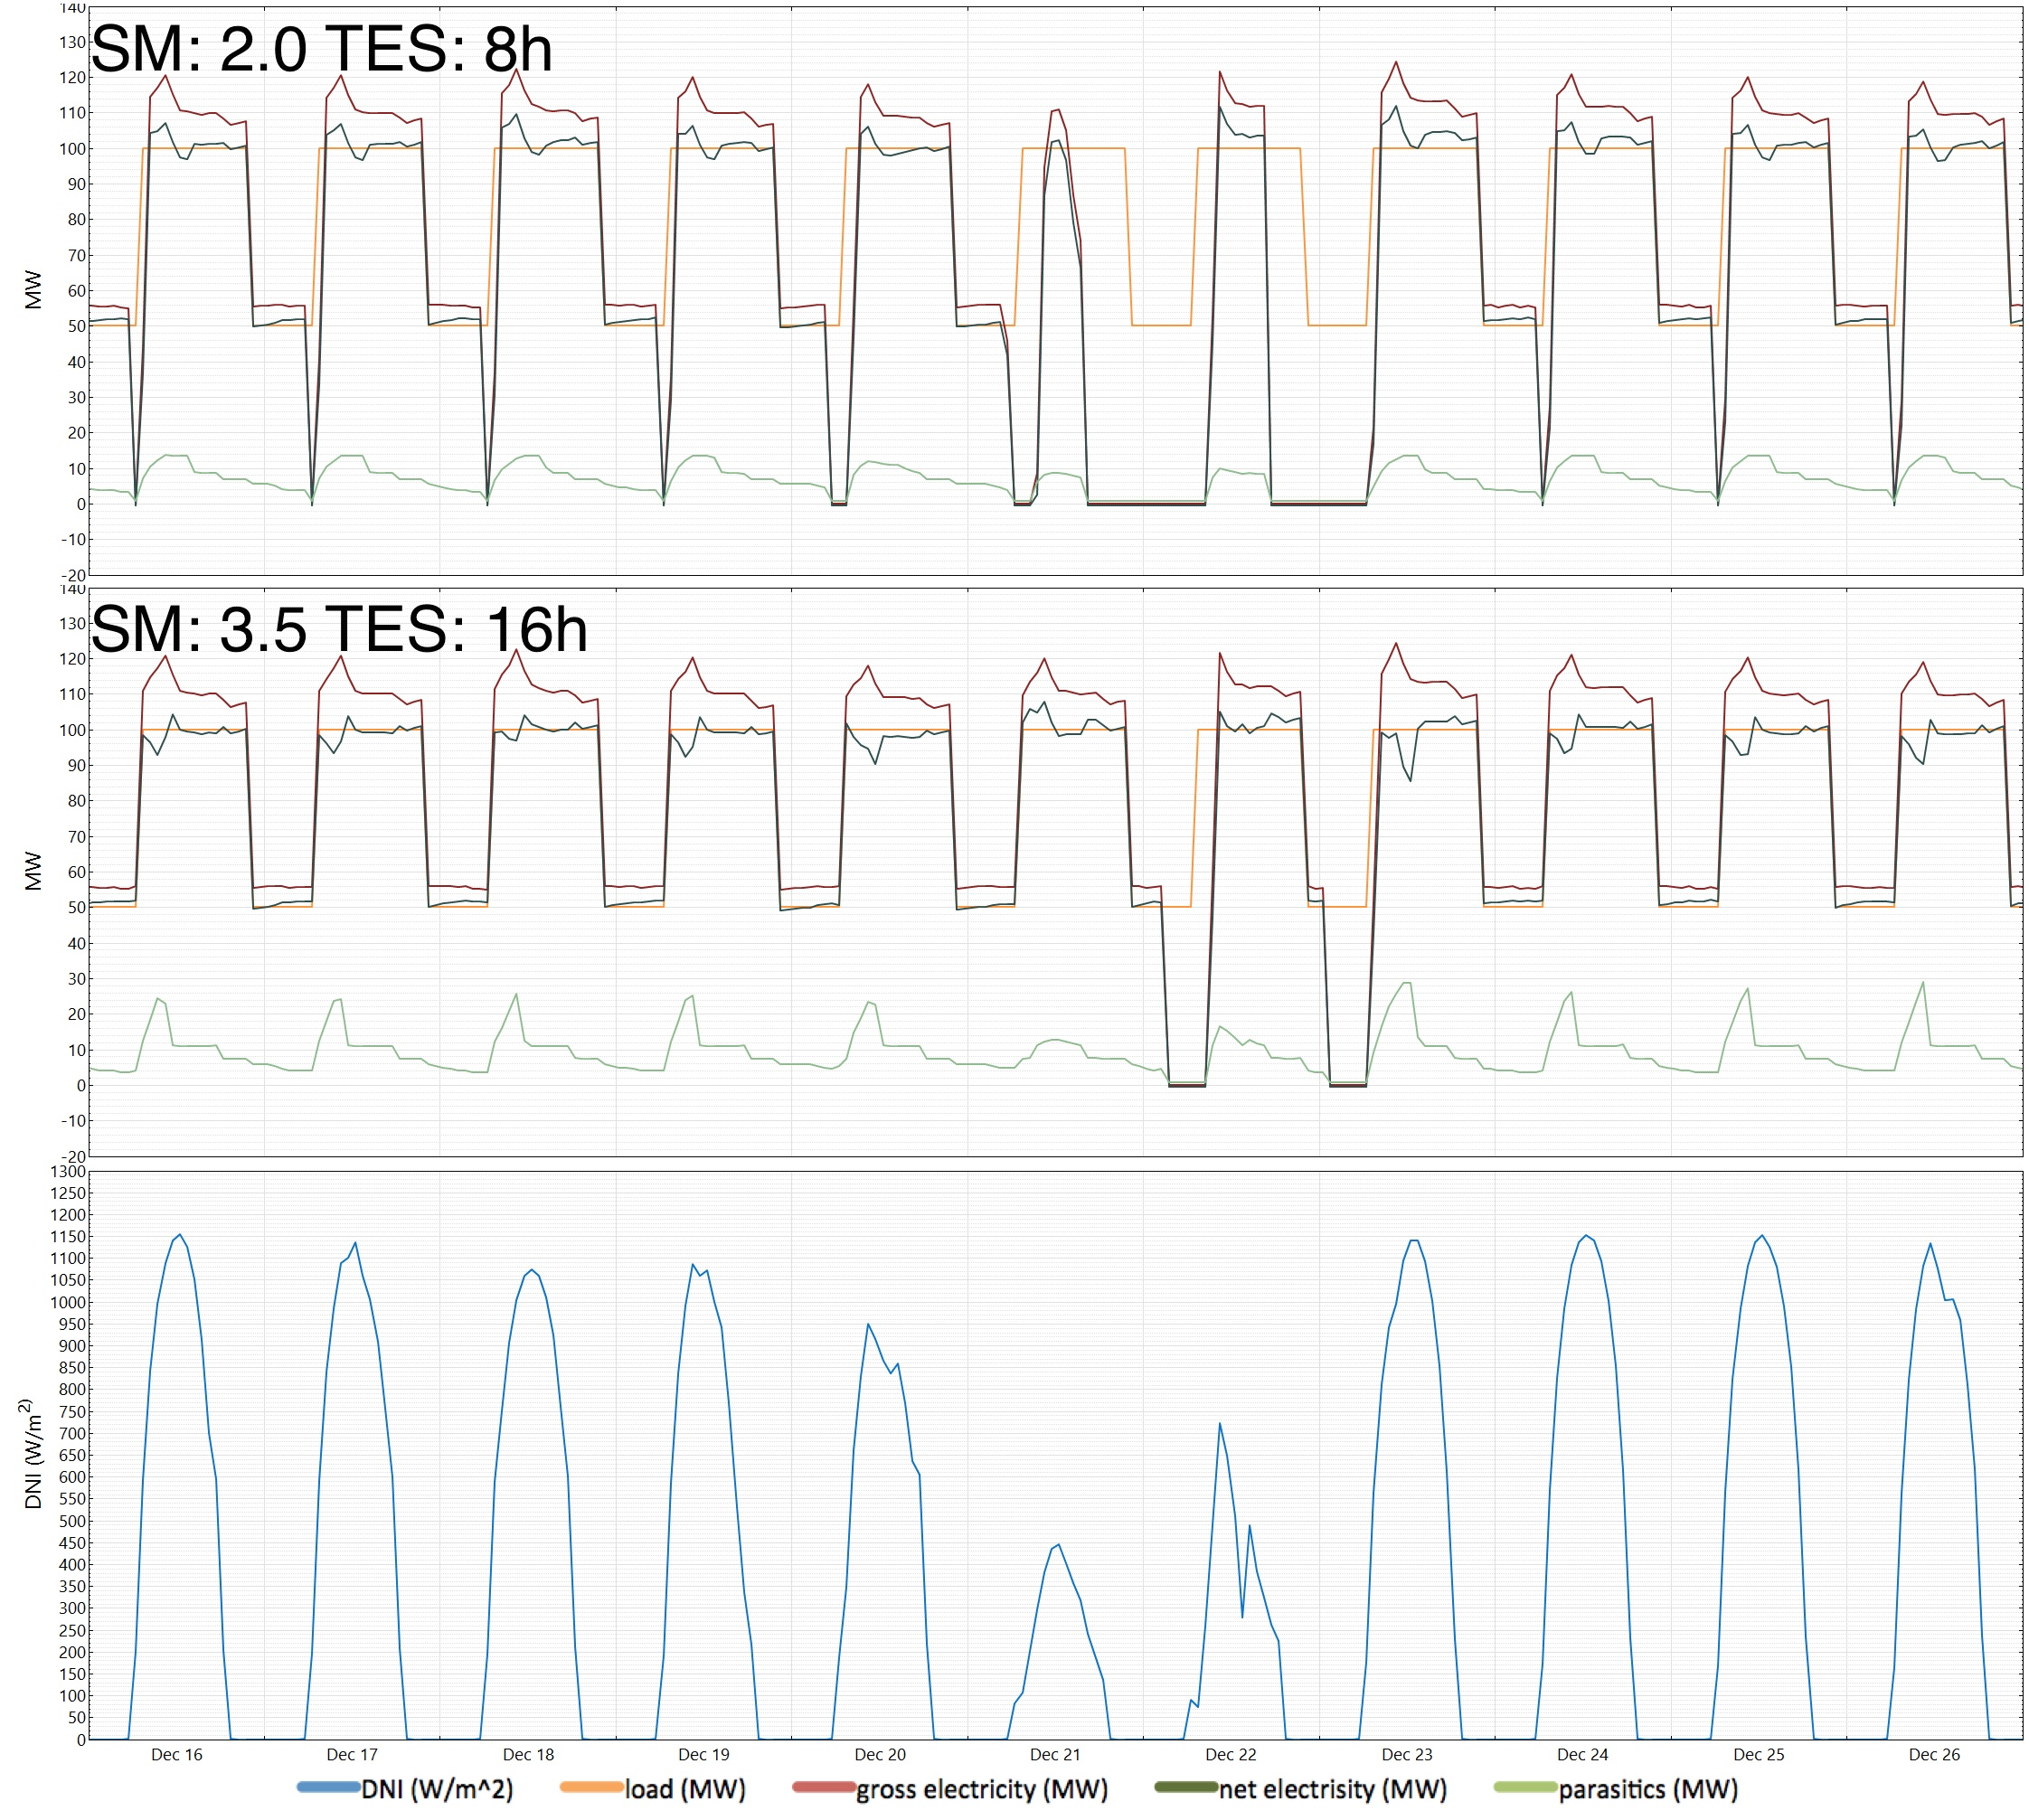
\includegraphics[width=1\linewidth]{FIG/CR_summer_load}
\caption[CR load profile during the time of summer solstice (16. December - 26. December).]{CR load profile during the time of summer solstice (16. December - 26. December).}\label{CR_summer_load}
\end{figure}
This leads also to the above mentioned decreasing in supply at \SI{8}{am} in the annual average load profile. The difference between the gross and net electricity production is coming from the parasitic consume within the power plant.

Figure~\ref{CR_summer_load} describes the load behavior of the  same power plants during the longest days of the year. It is clearly to see, that the irradiation is higher and longer during the days compare to the winter solstice. The peaks of DNI are about 1~\SI{150}{\watt\per\square\metre} during that days. At a SM of 2.0 and \SI{8}{h} of TES the CR power plant is not able to follow the prescribed electricity load over the whole day. It's coming to standstill between 6 and \SI{7}{am} at least. Therefrom also the annual average load profile is coming to stand still at these time of the day. The CR power plant with a SM of 3.5 and \SI{16}{h} of TES can follow the prescribed load mostly without any problems. Outstanding for the high productivity of the plant configuration is the electricity output while having low direct irradiance. At the 21. of December the plant can supply almost the whole prescribed load using reserves from the TES.

A detailed look to the parasitic behaviors of the CR power plant with a SM of \si{3.5} and \SI{16}{h} of TES reveals a strong decreasing after a moderate increasing during the midday. This happens when the storage is full loaded and the steam turbine don't need more power. At this point a specified amount of heliostats defocusing the receiver and the power of the receivers HTF pump is getting reduced. 

\begin{figure}[!htbp]
        \centering   
        \begin{subfigure}[b]{0.65\textwidth}
                \centering
                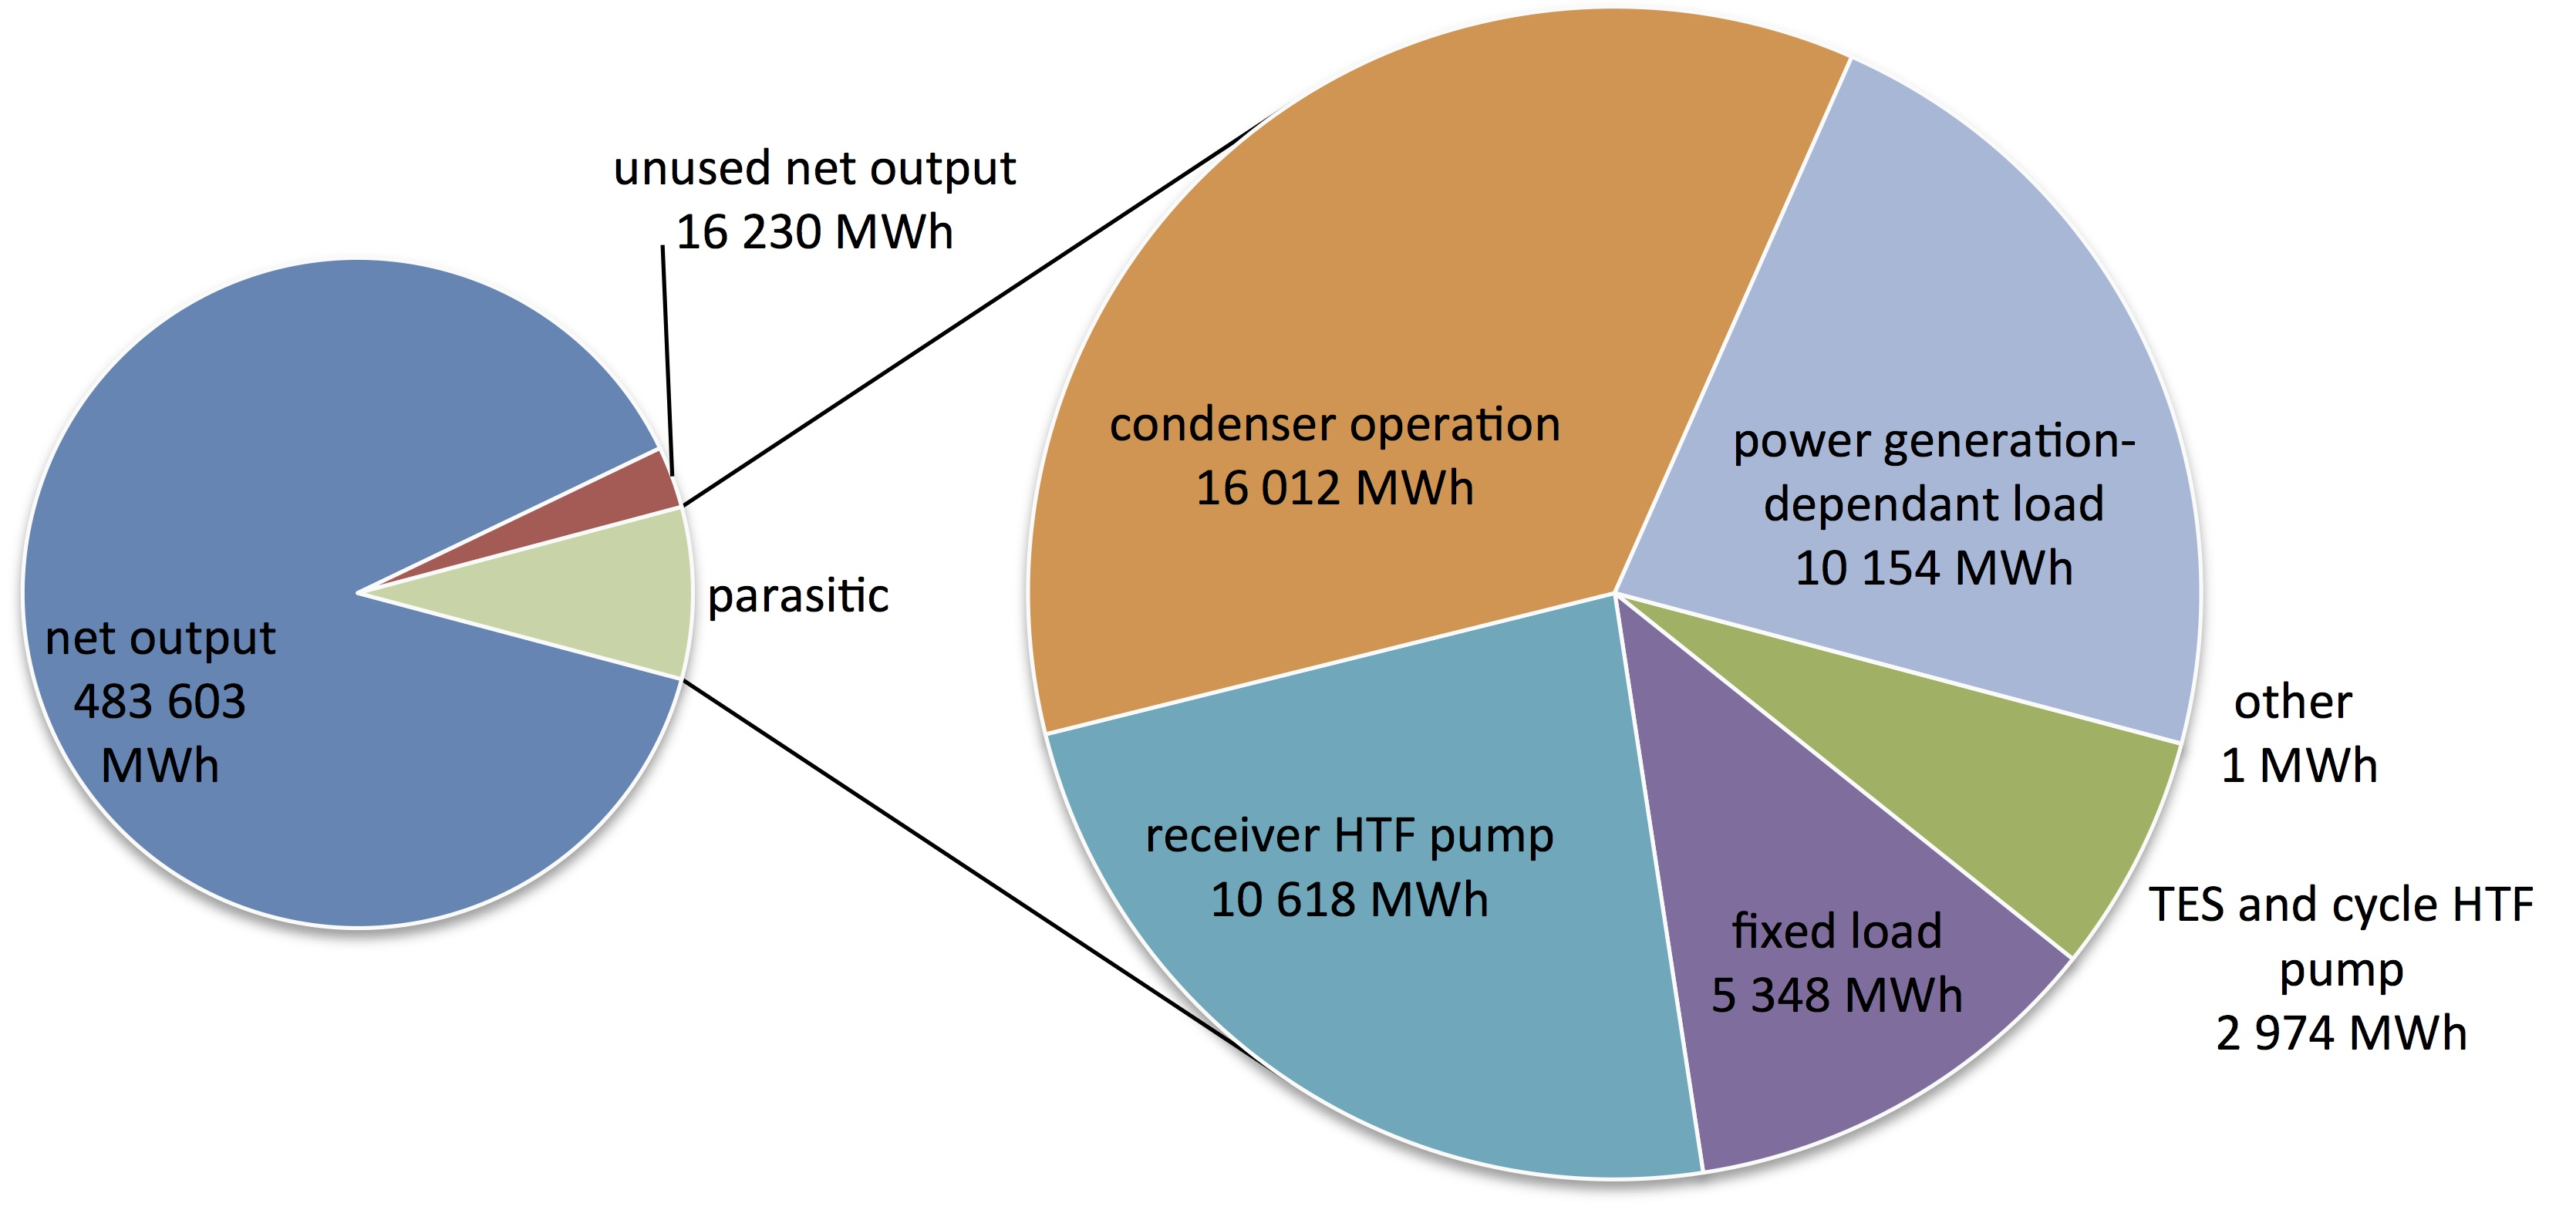
\includegraphics[width=1\textwidth]{FIG/CR_parasitics_low}
                \caption{SM: 2.0 TES: 8 h}\label{CR_parasitics_low}
        \end{subfigure}
\par\medskip % Linebreak              
        \begin{subfigure}[b]{0.65\textwidth}
                \centering
                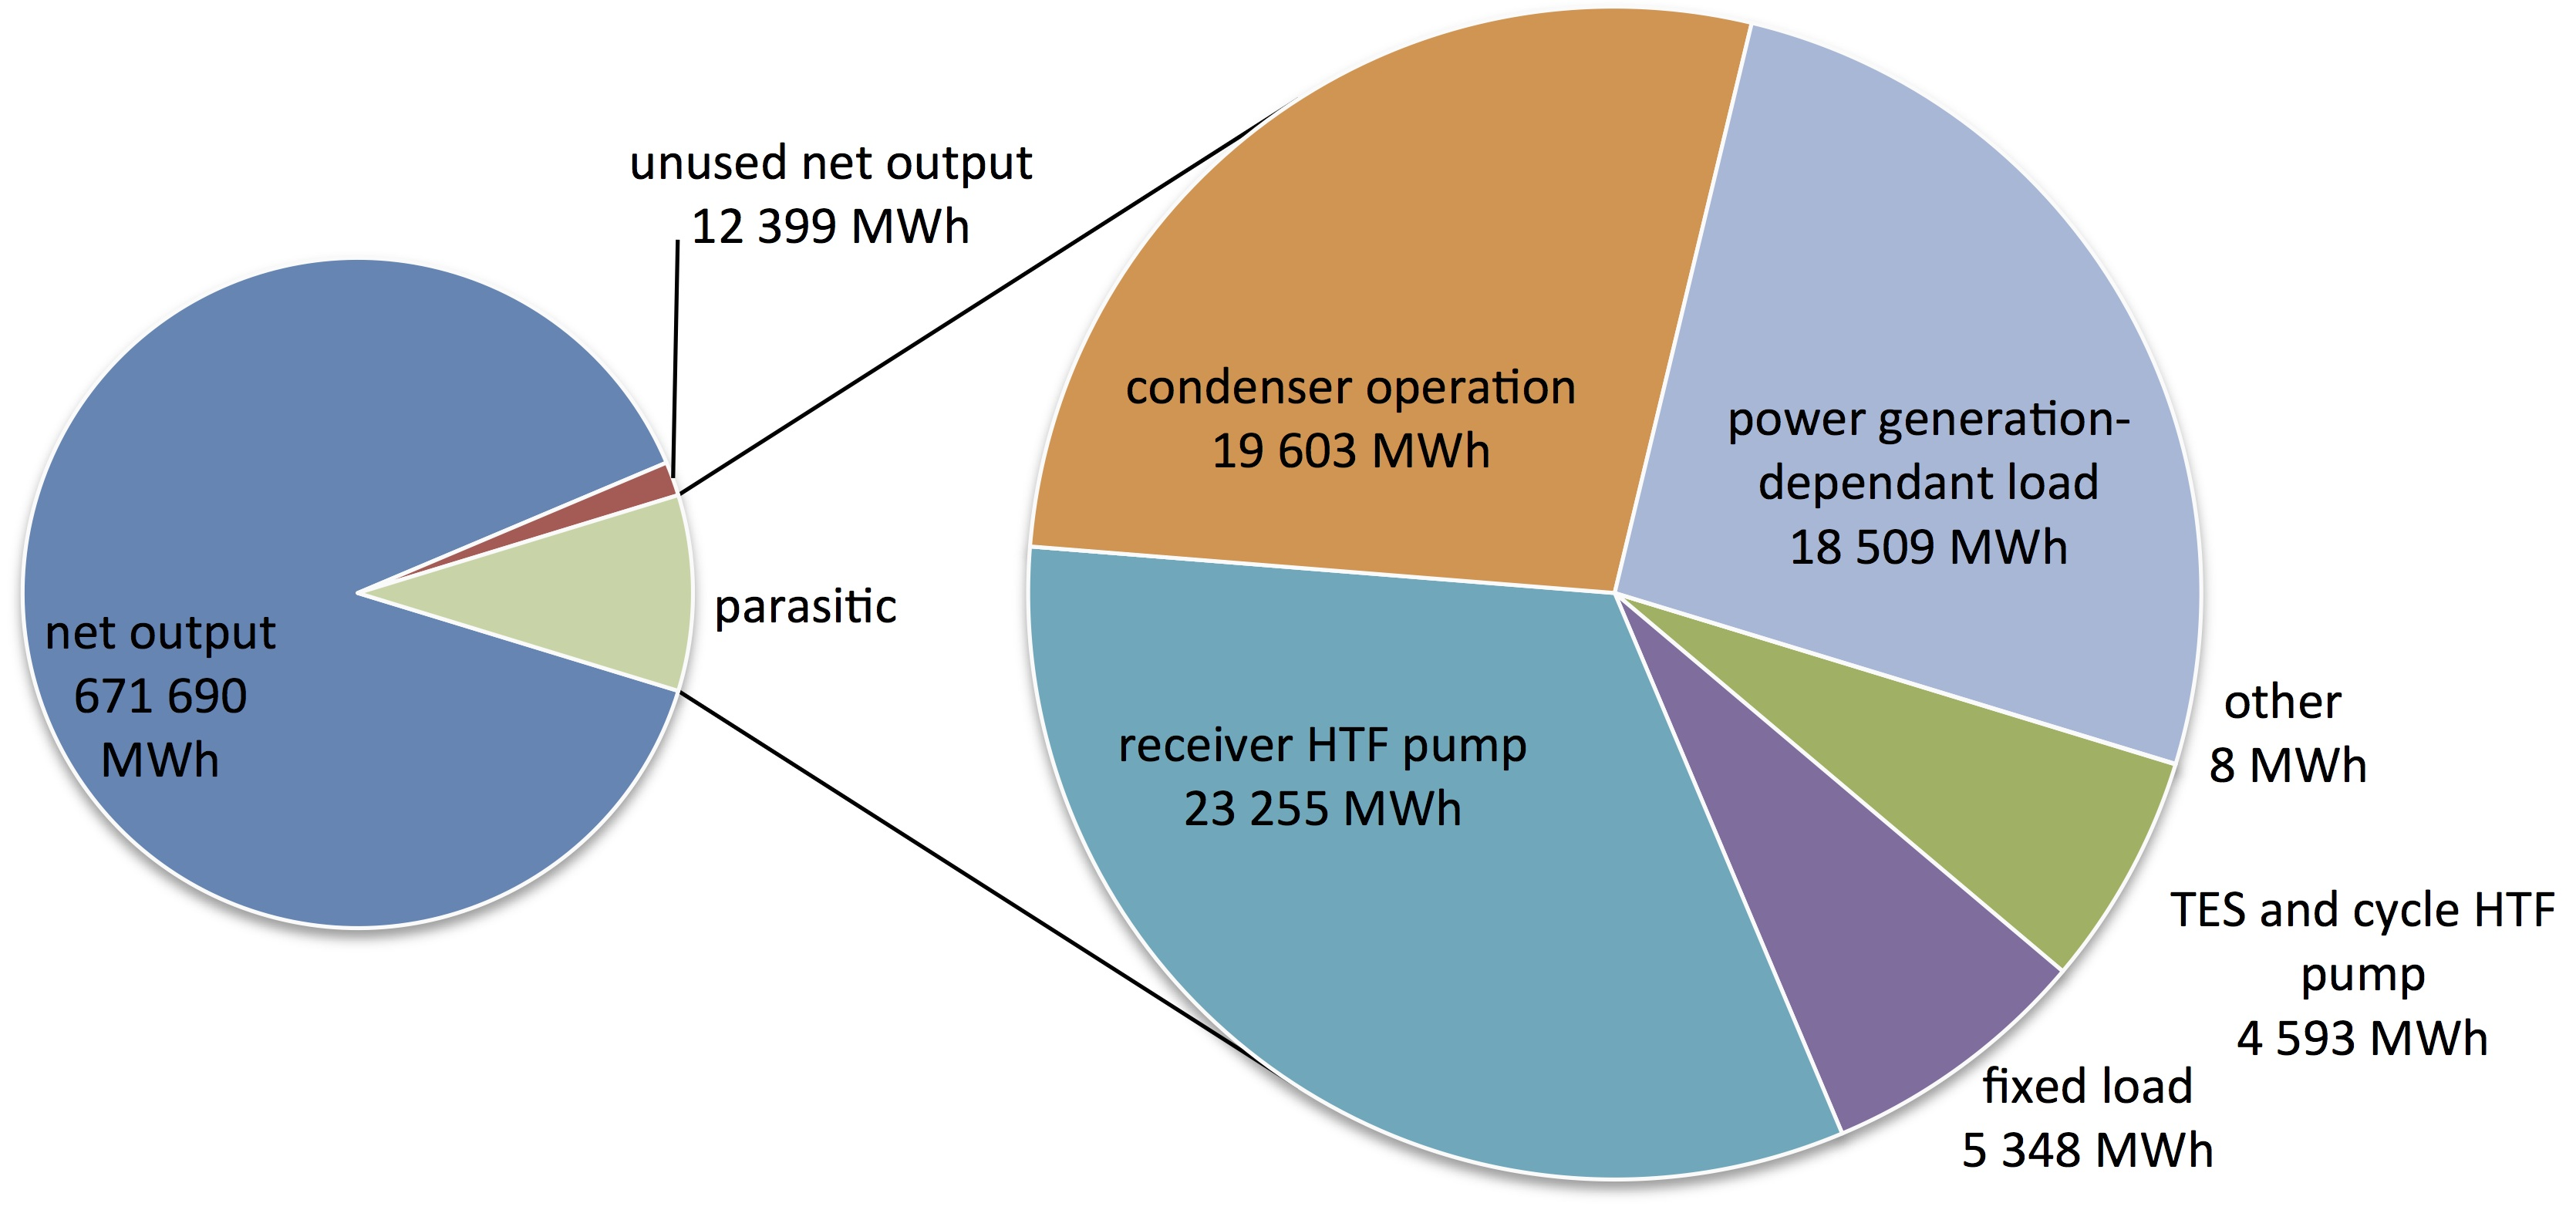
\includegraphics[width=1\textwidth]{FIG/CR_parasitics_high}
                \caption{SM: 3.5 TES: 16 h}\label{CR_parasitics_high}
        \end{subfigure}
        \caption[Share of annual gross energy output of selected CR power plant configurations.]{Share of annual gross energy output of selected CR power plant configurations.}\label{CR_parasitics}
\end{figure}
The parasitic load is composed from various electrical loads of the power plant, namely pumping loads, cooling loads, fixed loads and loads depending from the power generation. The share of these electrical parasitic loads and the total share of the gross energy output of the selected CR power plans can be seen in Figure~\ref{CR_parasitics}. The share of the net energy production out of the gross energy production is about 90~\%. The unused net energy output share of all simulated CR power plants is between 1.6 and 3.2~\% and went not into the LCOE calculation.

Figure~\ref{CR_parasitics_low} shows, that the net outputs share of the lowest CR power plant configuration is about \SI{483.60}{GWh}.  The total sum of the annual prescribed load is \SI{711.75}{GWh}. So the power plant covers the prescribed load for 67.9~\%. The net outputs share of the highest CR power plant configuration from Figure~\ref{CR_parasitics_high} is \SI{671.69}{GWh} and is covering the prescribed load for 94.4~\% over the year.

Figure~\ref{CR_LCCF} summarizes the results of the load curve covering for all simulated CR configurations. The chart shows that at a SM of 2.0 all TES variations besides \SI{8}{h} a covering more than 70~\% of the prescribed load. At a SM of 2.5 the and a TES about \SI{10}{h} the results showed over 80~\% load covering. A load curve covering of about 90~\% is reached at a SM of 3.0 and more than \SI{14}{h} of TES. The configuration with a \SI{12}{h} TES reaches just 89.1~\% at a SM of 3.0. 

\begin{figure}[htbp]  
\centering
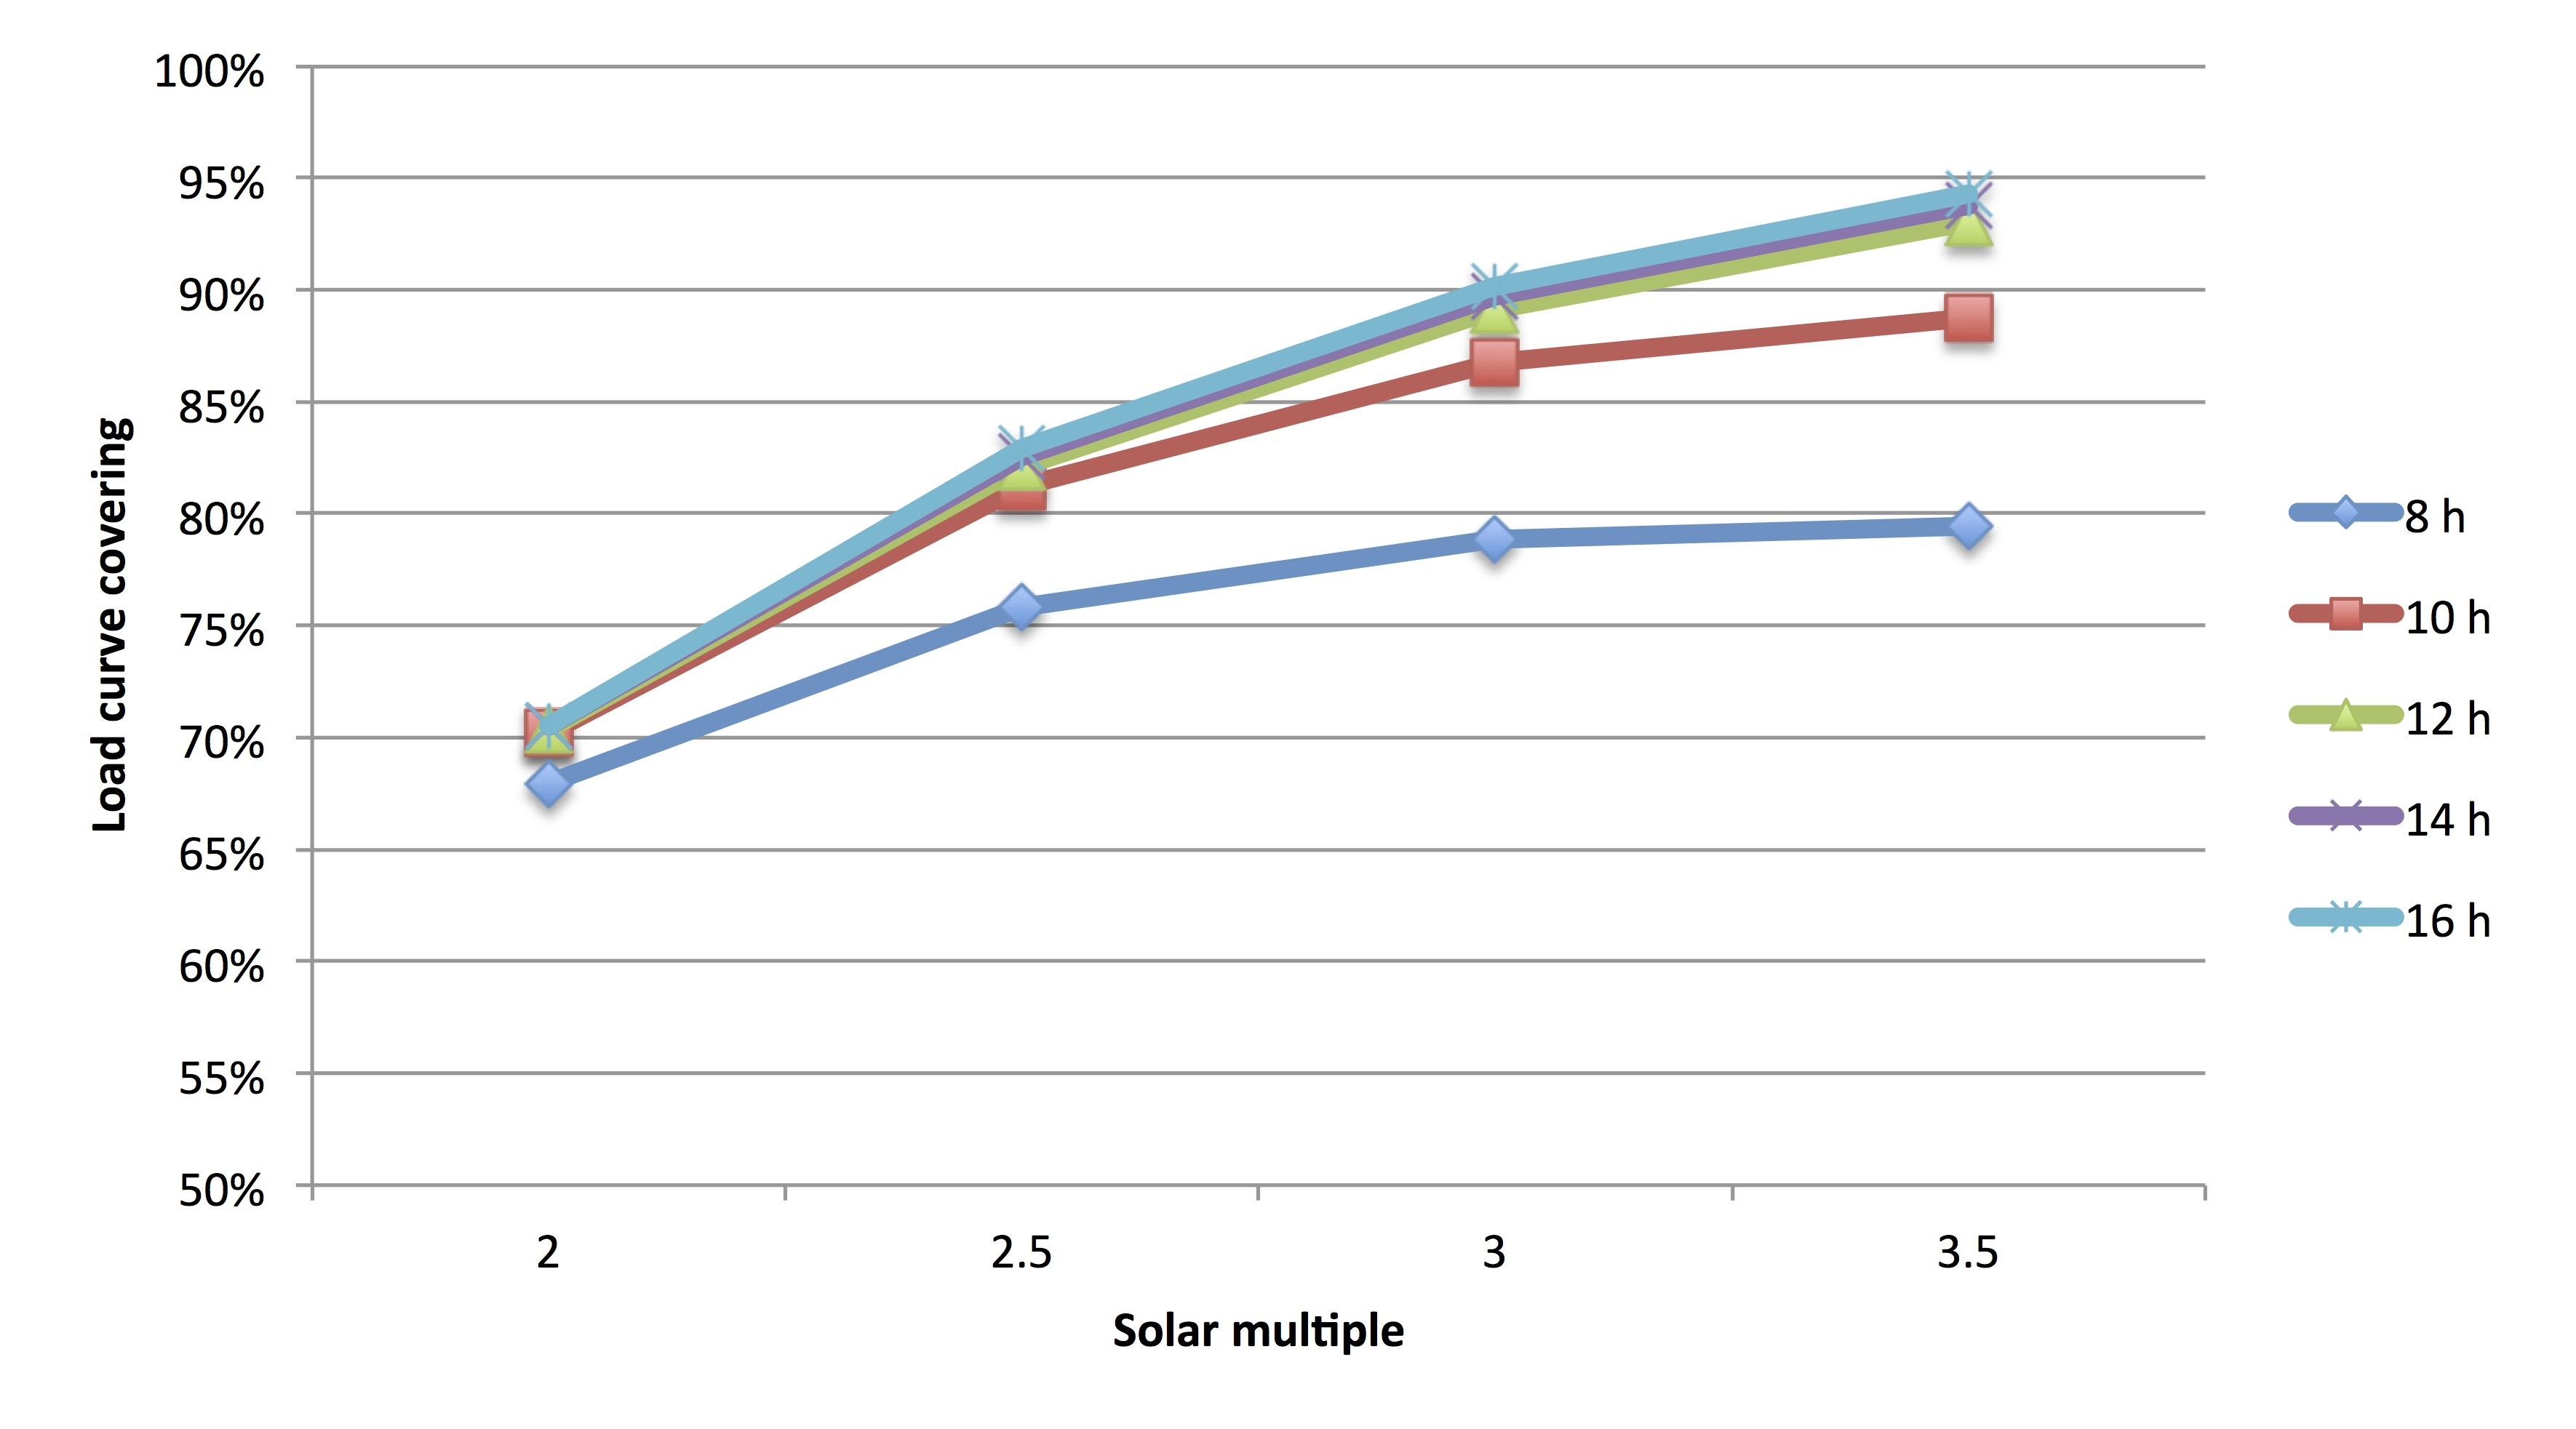
\includegraphics[width=1\linewidth]{FIG/CR_LCCF}
\caption[Load curve covering result of simulated CR systems.]{Load curve covering result of simulated CR systems.}\label{CR_LCCF}
\end{figure}
The results of the load curve covering shows that there is no appreciable difference between the 12, 14 and \SI{16}{h} of TES. At a SM of 3.5 the difference is just 1.4~\% load curve covering between 12 and \SI{16}{h} of TES. There is just a addition of 0.6~\% for the \SI{8}{h} TES and the SM 3.0 to 3.5 configurations. 
\subsubsection{Levelized costs of electricity}
The results of the LCOE claculation for the simulated CR configurations can be seen in Figure~\ref{CR_LCOE}. They are calculated using the finacial input parameter in Table~\ref{tbl: CRFinance} and a simplified method which is documented in Appendix~\ref{ChapterLCOE} on Page \pageref{ChapterLCOE}.

\begin{figure}[htbp]  
\centering
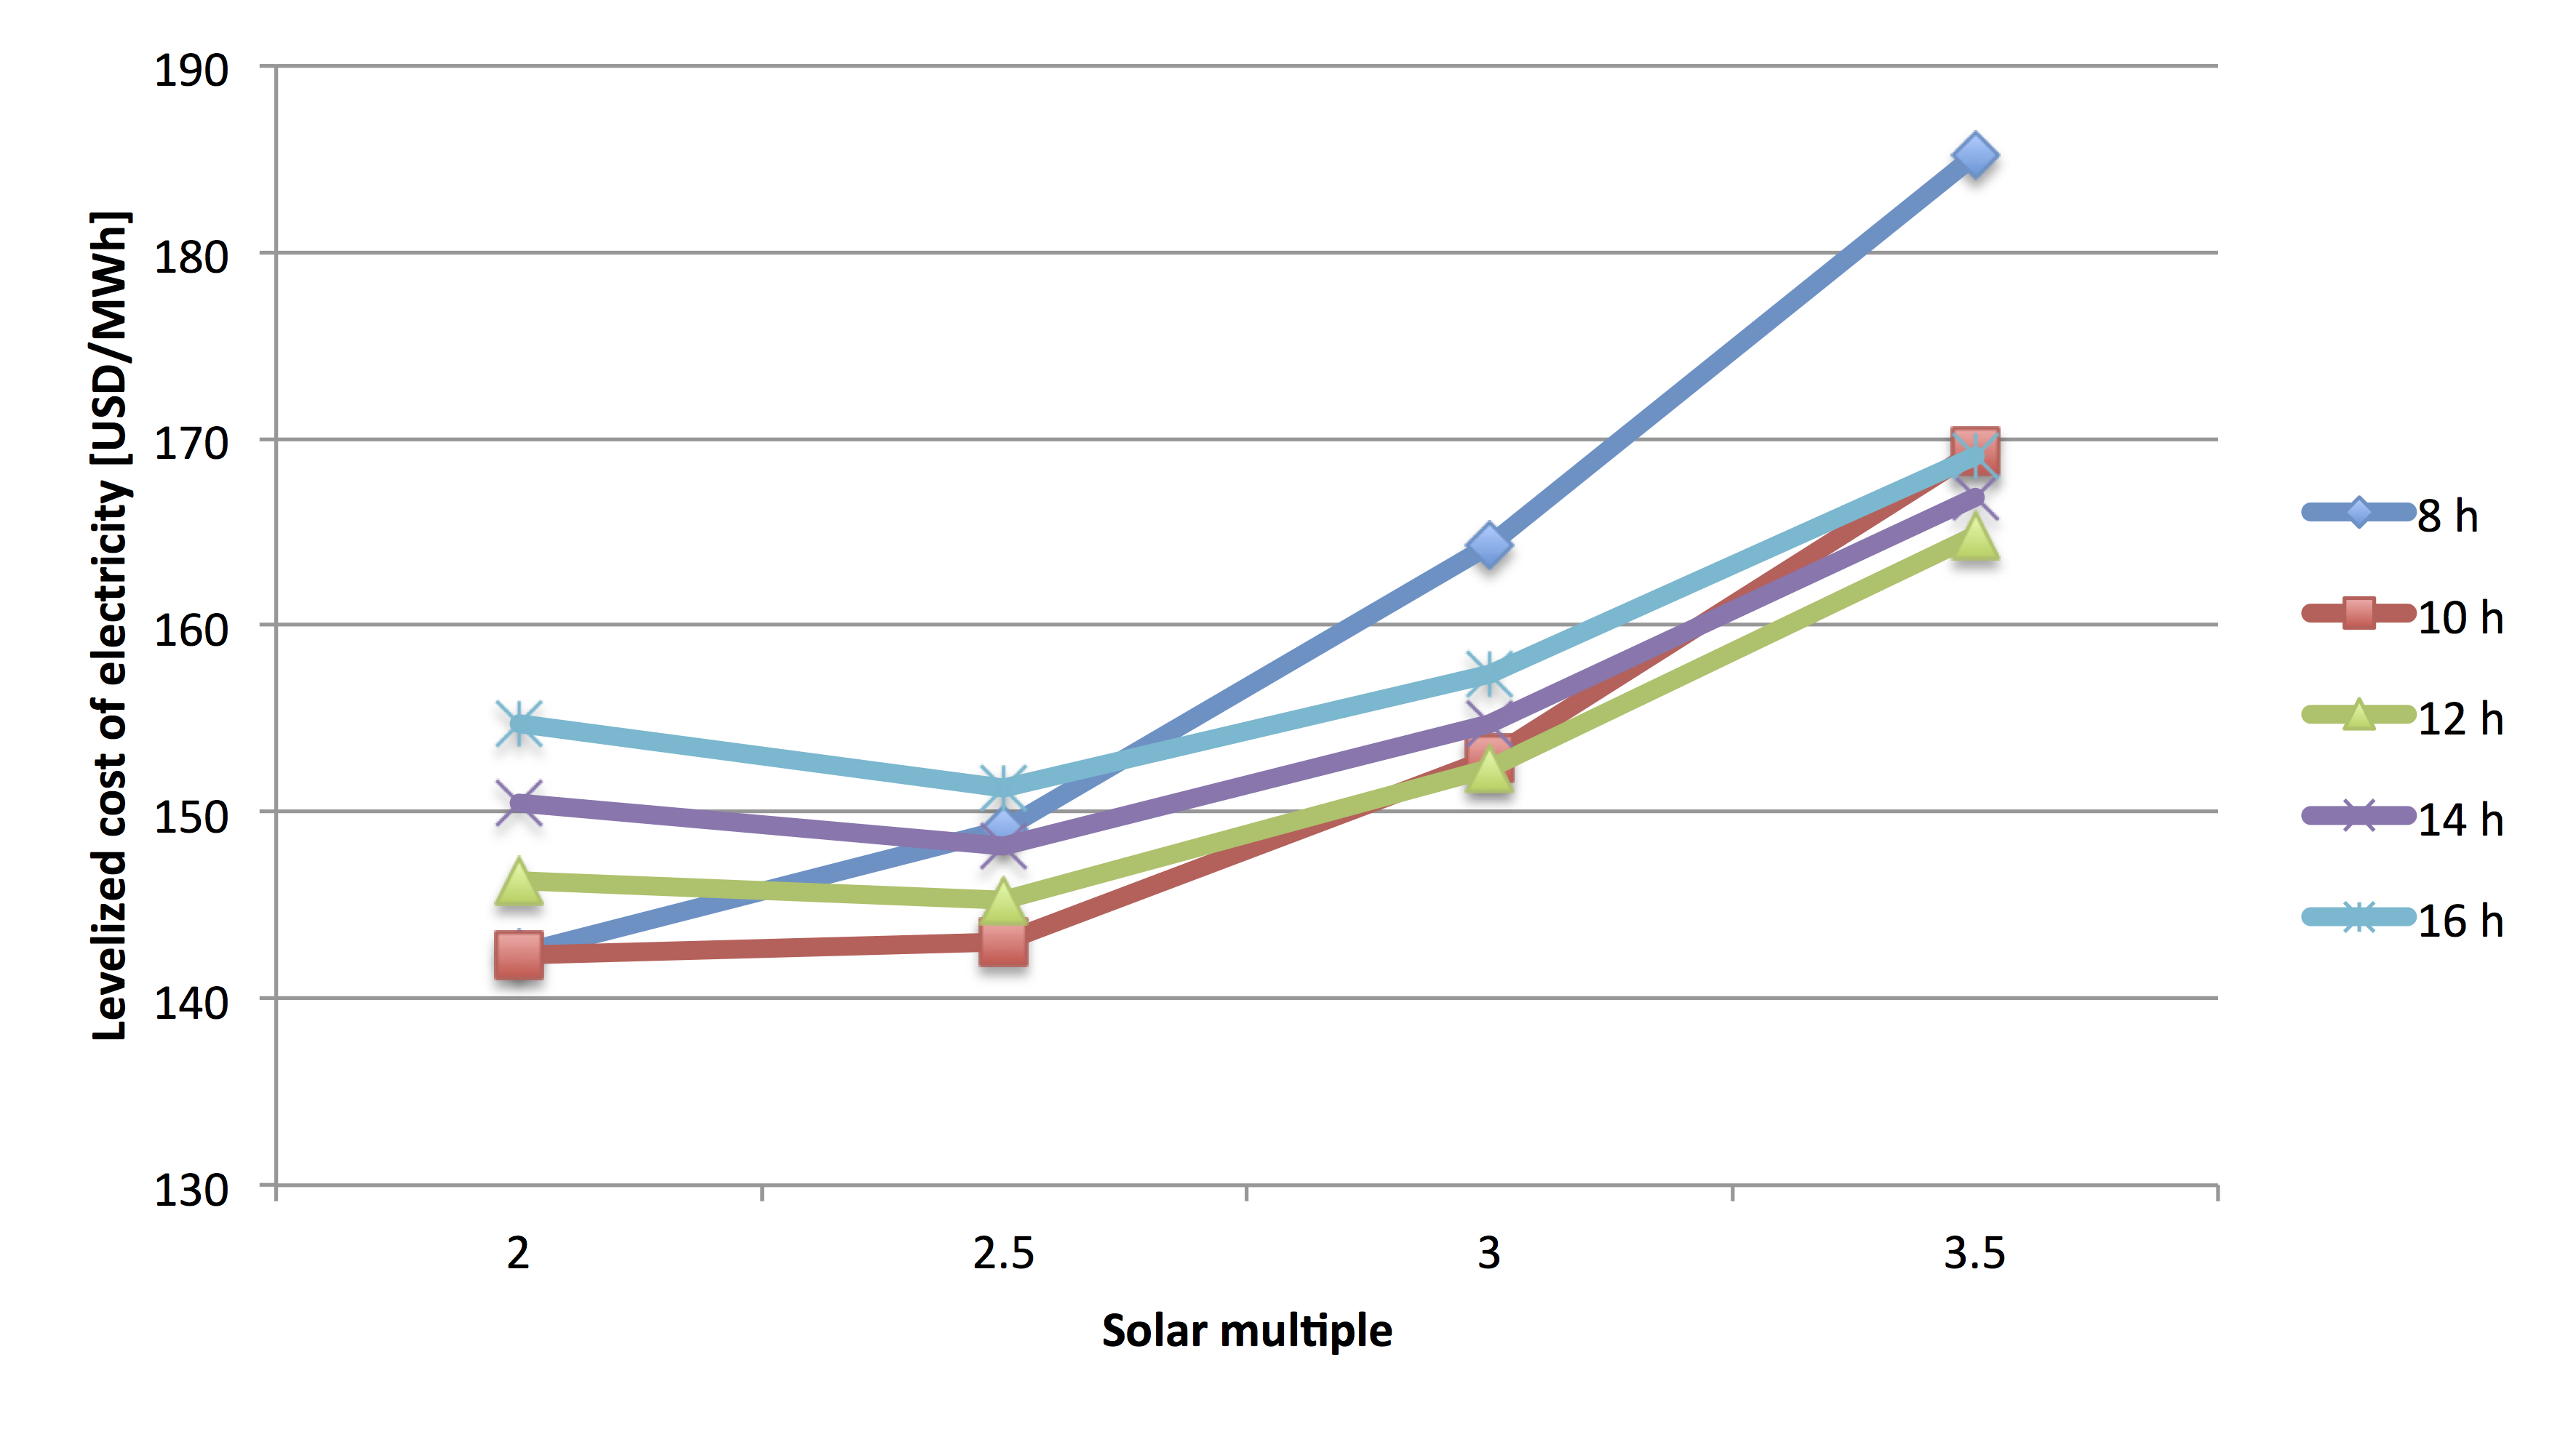
\includegraphics[width=1\linewidth]{FIG/CR_LCOE}
\caption[LCOE calculation results for CR simulation.]{LCOE calculation results for CR simulation.}\label{CR_LCOE}
\end{figure}
The results of the calculation shows that the lowest LCOE of \SI{137.55}{USD/MWh} is reached at a SM of 2.0 and \SI{10}{h} of TES and is just  marginal cheaper then using \SI{8}{h} of TES with a LCOE of \SI{137.63}{USD/MWh}. The LCOE addition from SM 2.0 to 2.5 is goes minimal up to \SI{138.25}{USD/MWh} for \SI{10}{h} of TES. The highest LCOE result of the simulated configurations is \SI{179.00}{USD/MWh} at a SM of 3.5 and \SI{8}{h} of TES. 

The behavior of the 12, 14 and \SI{16}{h} of TES results for all SM of the LCOE is almost identical. Just the individual value is differently.

\begin{figure}[!htbp]
        \centering                
        \begin{subfigure}[b]{0.5\textwidth}
                \centering
                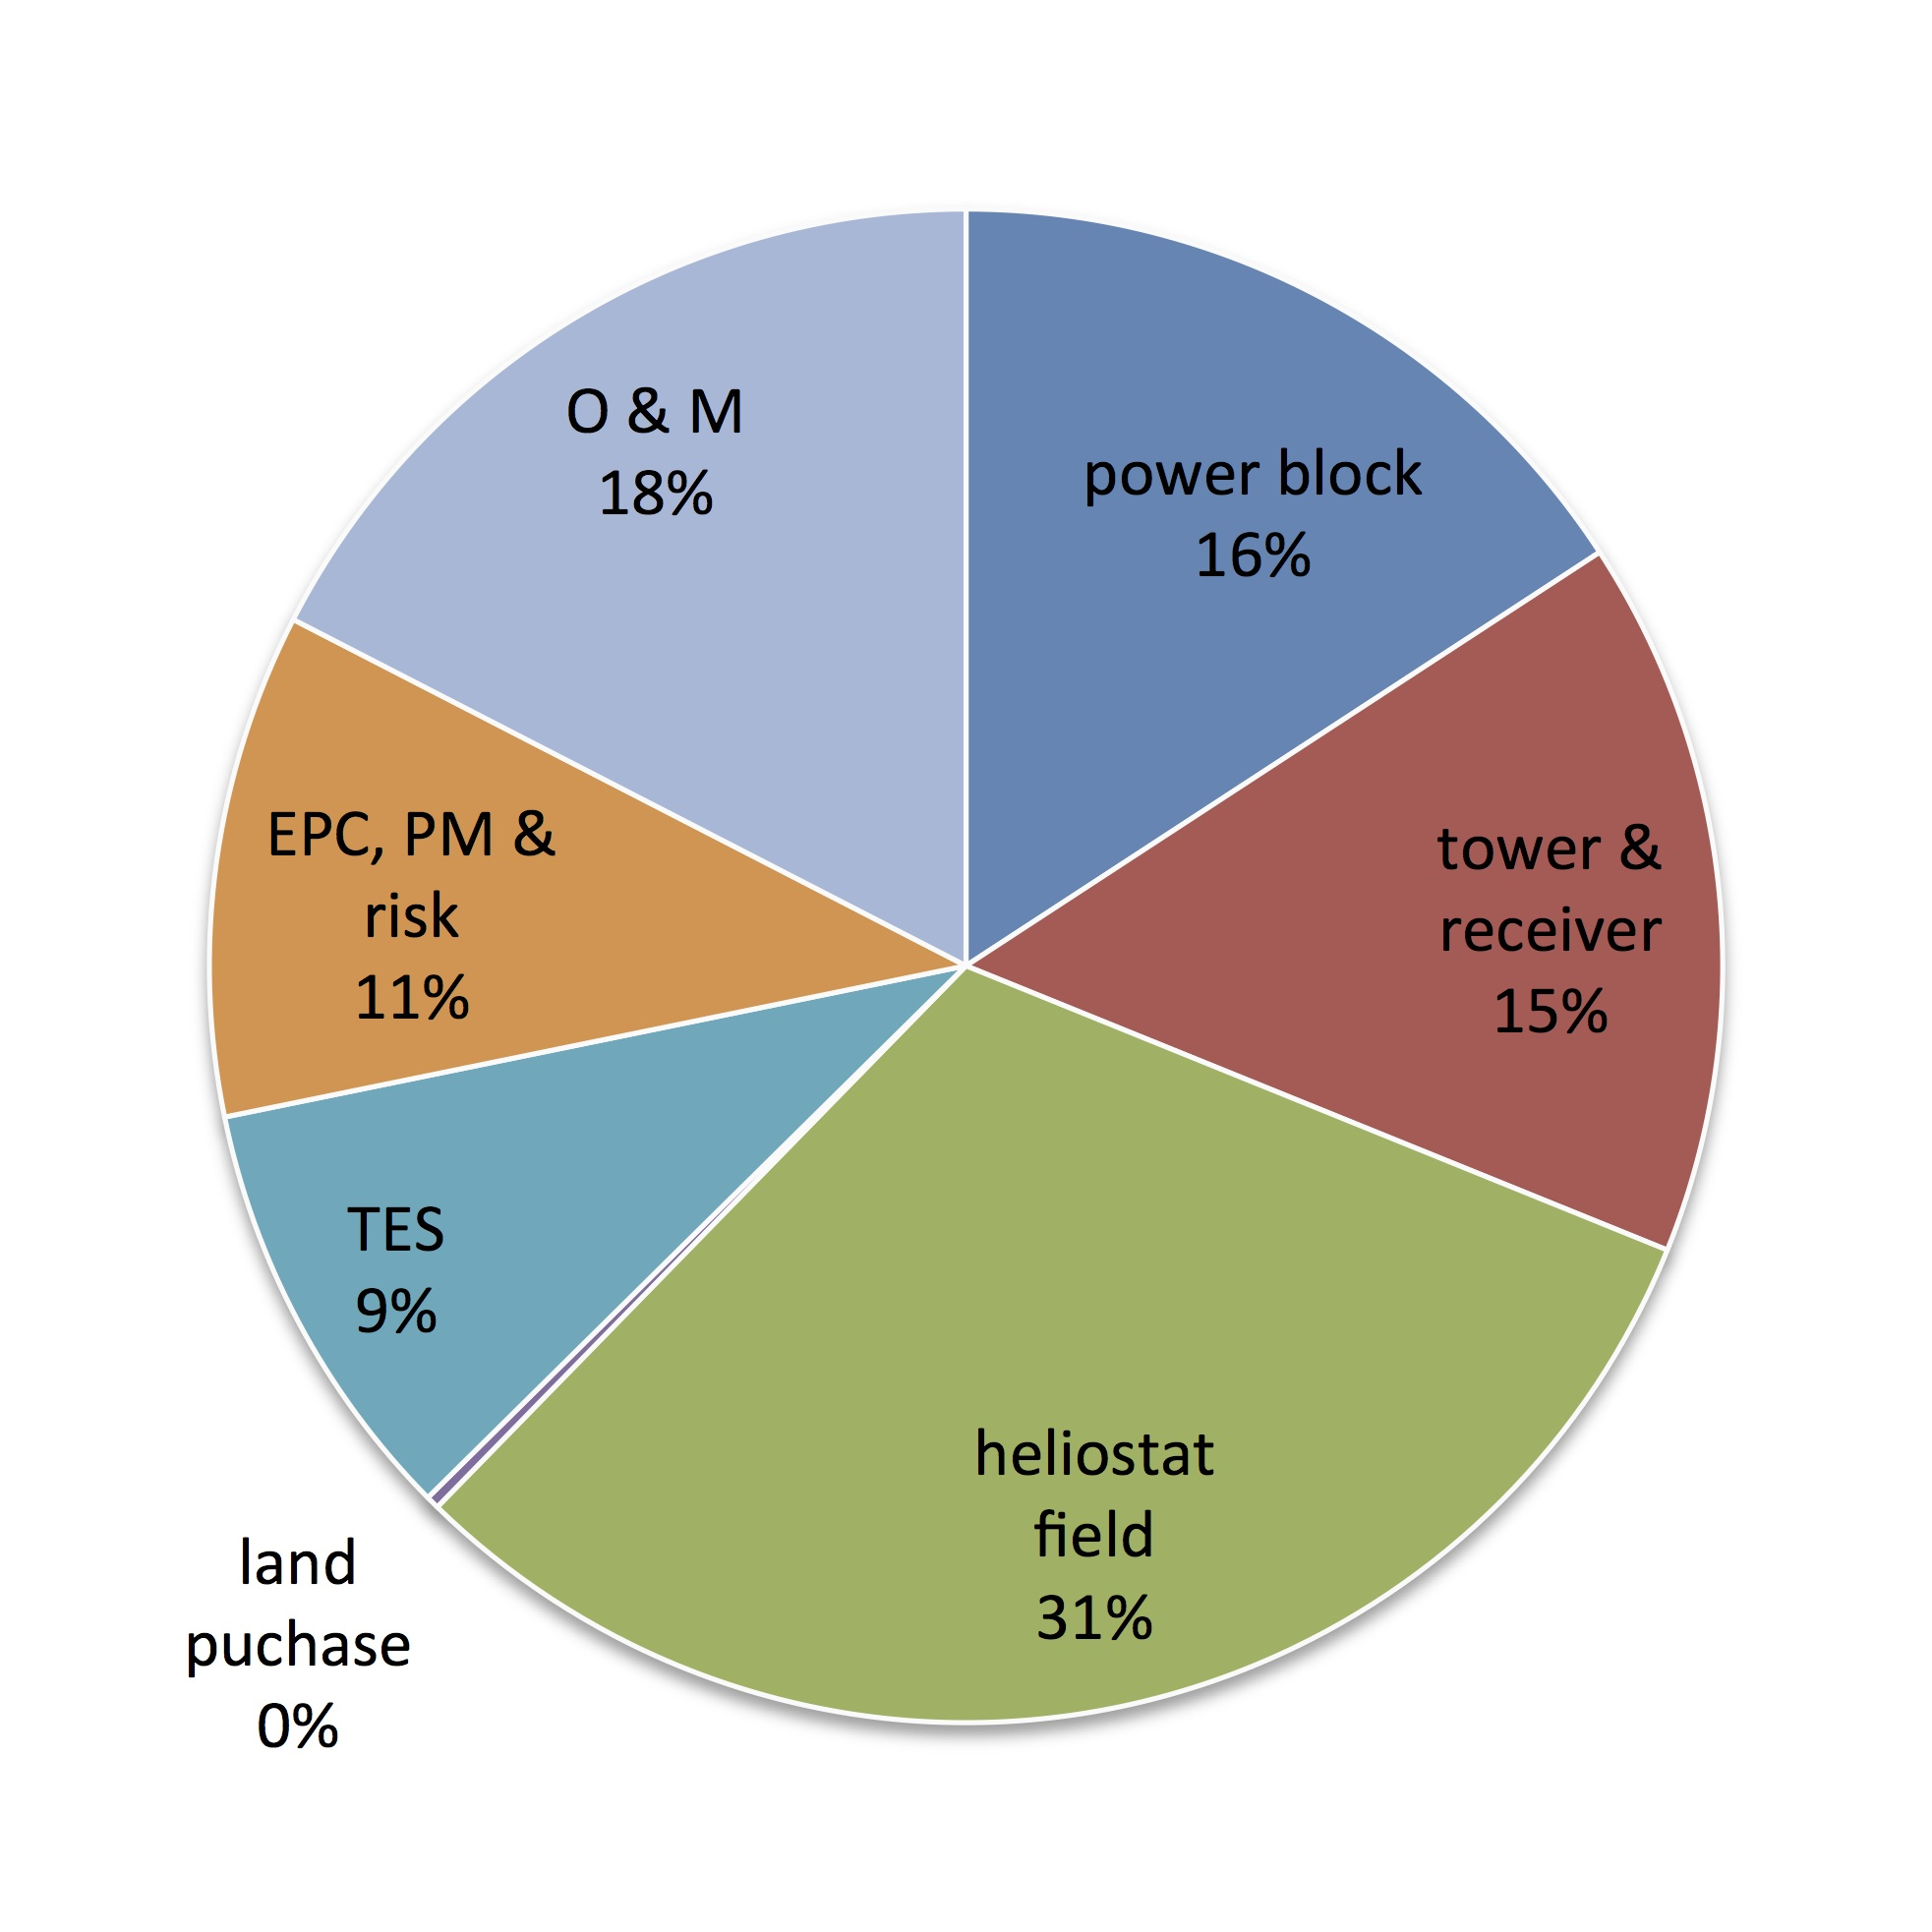
\includegraphics[width=1\textwidth]{FIG/CR_LCOE_lowinvest_BreakDown}
                \caption{LCOE break-down for SM~2.0 and \SI{8}{h}~TES.}\label{CR_LCOE_lowinvest_BreakDown}
        \end{subfigure}%
        ~
        \begin{subfigure}[b]{0.5\textwidth}
                \centering
                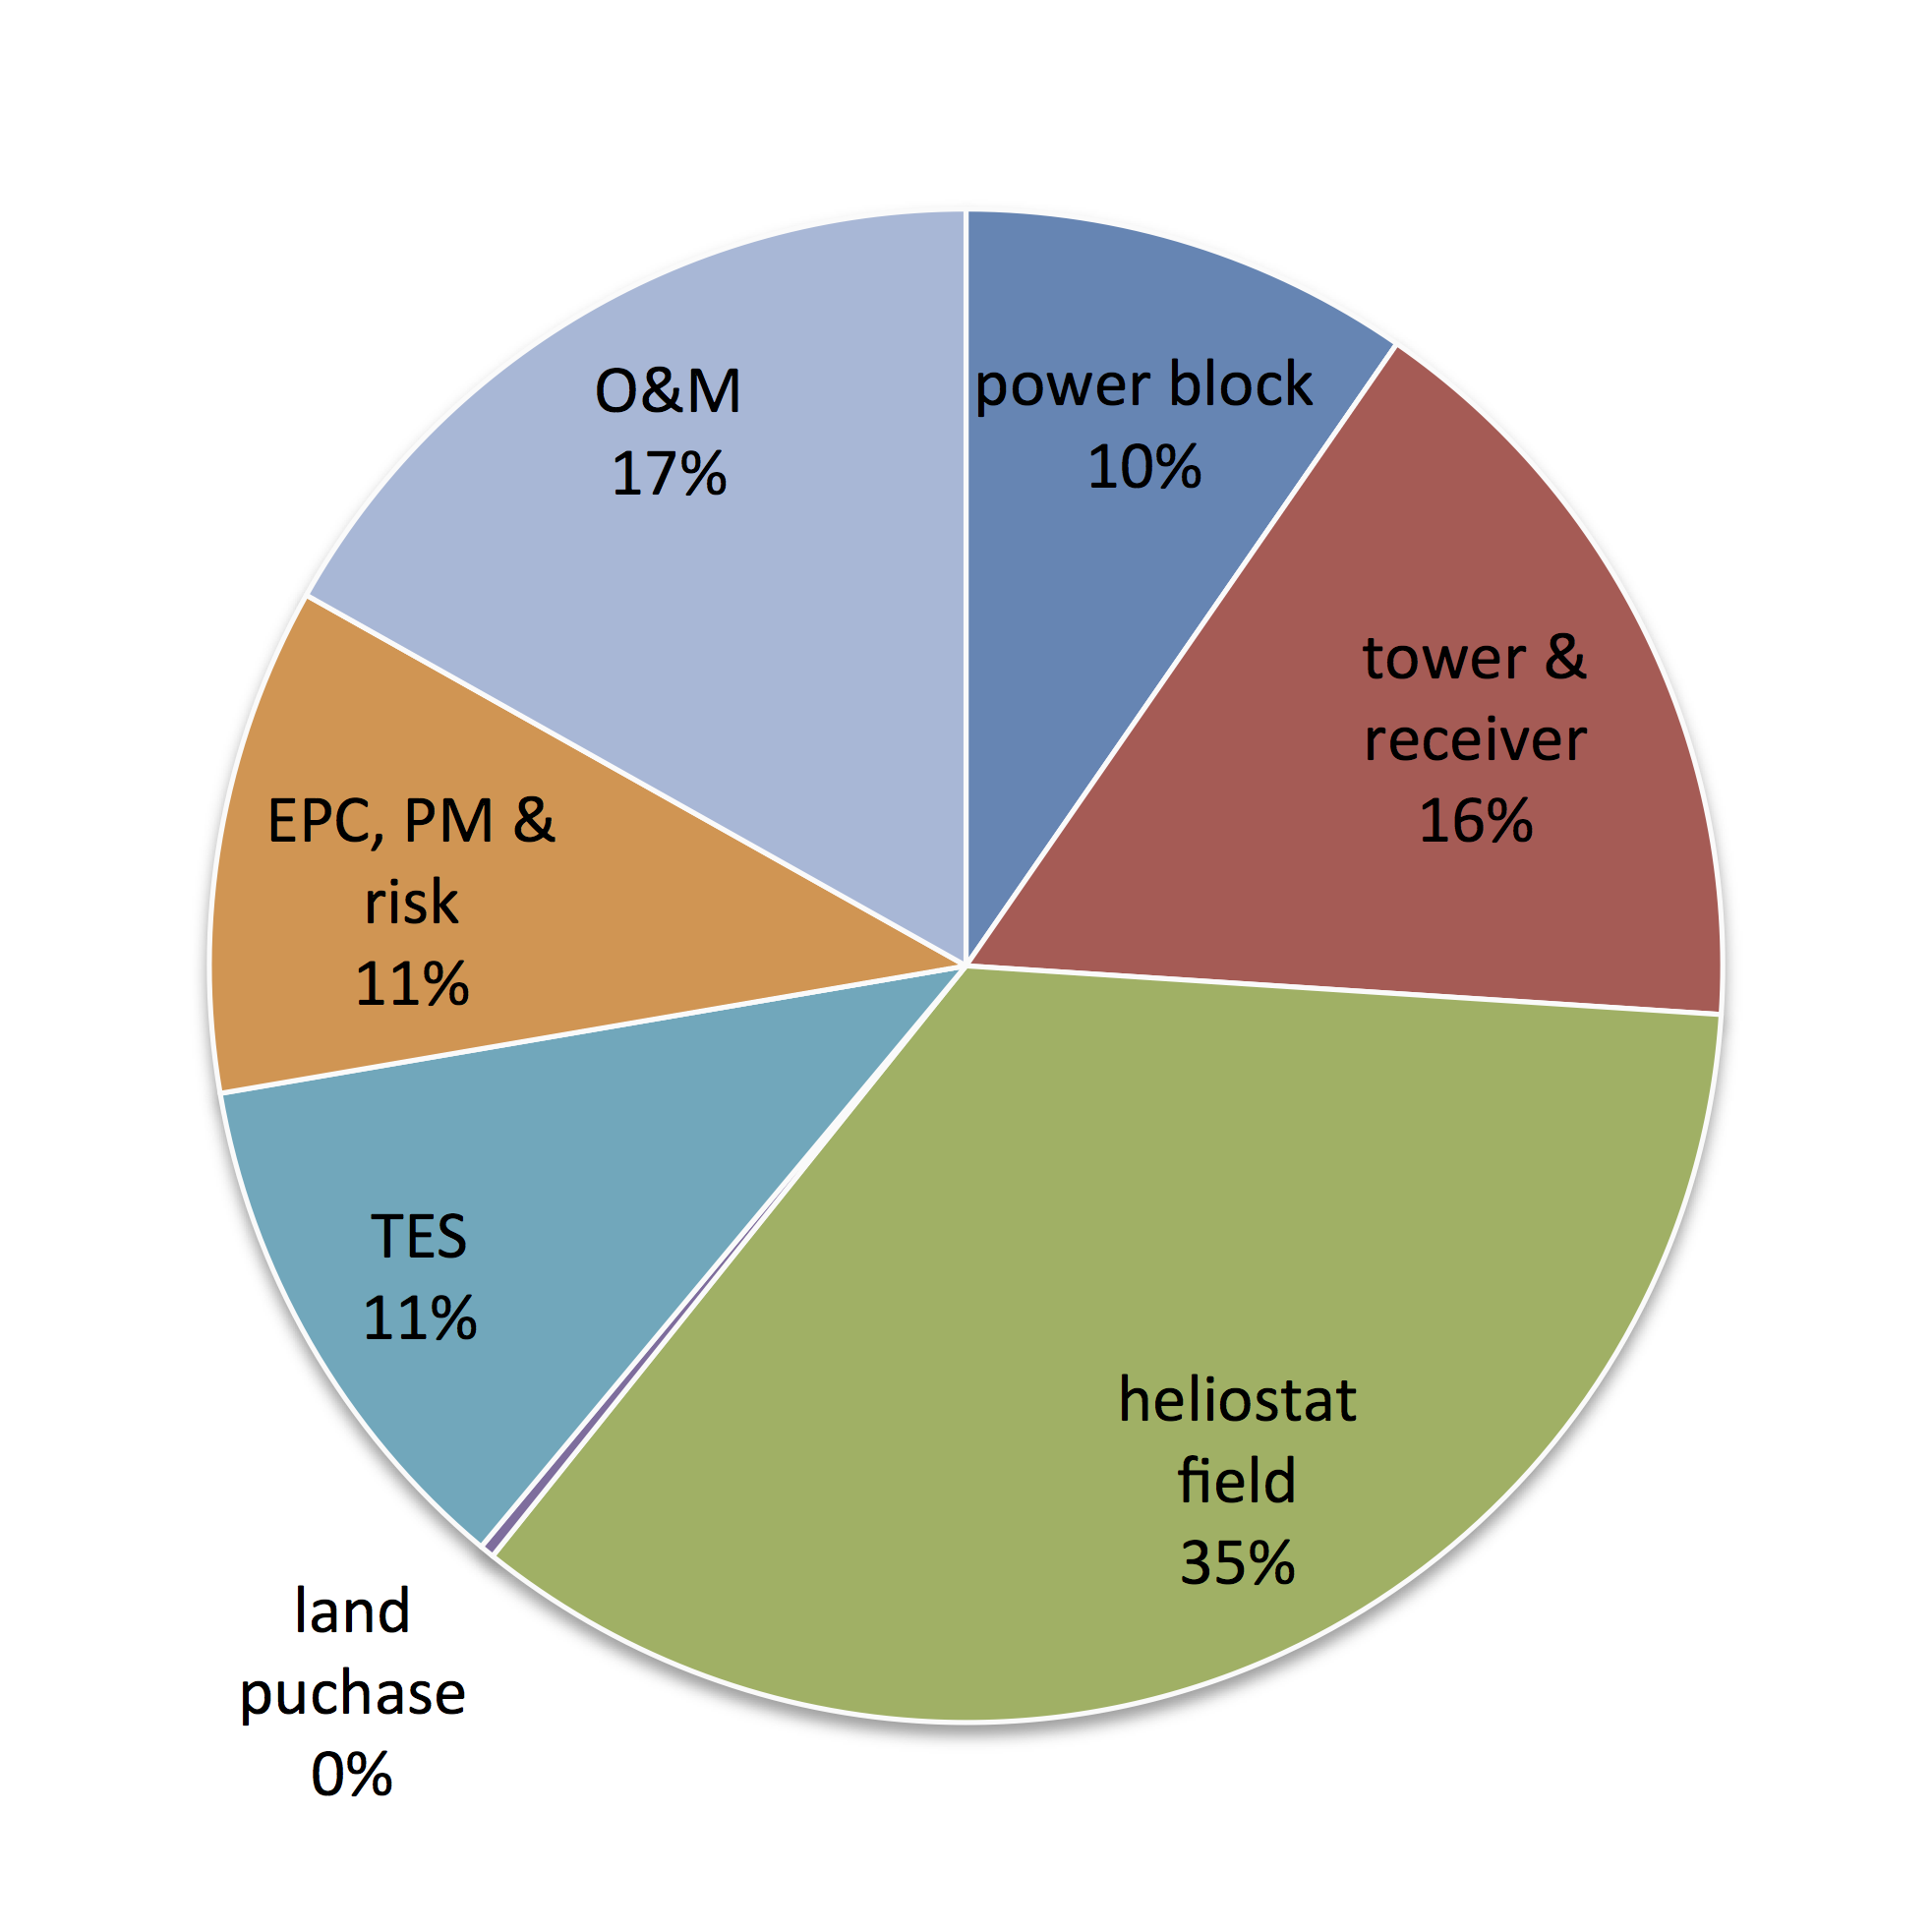
\includegraphics[width=1\textwidth]{FIG/CR_LCOE_highinvest_BreakDown}
                \caption{LCOE break-down for SM~3.5 and \SI{16}{h}~TES.}\label{CR_LCOE_highinvest_BreakDown}
        \end{subfigure}
        \caption[Break-down of selected CR-LCOE calculation results.]{Break-down of selected CR-LCOE calculation results.}\label{CR_LCOE_BreakDown}
\end{figure}
The calculated LCOEs of the simulated CR power plants is composed by seven cost parts. The investment costs of power block, tower and receiver, heliostat field, land purchase, TES, additional EPC, project management (PM) and risk as well as the annual costs for operation and maintain (O\&M). The brake-down of the LCOE components can be seen in Figure~\ref{CR_LCOE_BreakDown} for the simulation of the lowest and the highest configuration.  It can be seen that the investment costs of the land purchase don't have any influence to the LCOE of the simulated CR configurations. Also the share of the EPC, PM and risk as well as the share of O\&M don't varies much.

When comprising the results of the load curve covering with the LCOE calculation the lowest LCOE for reaching the target of 90~\% is the configuration of a SM of 3.0 and \SI{14}{h} of TES. The LCOE for these configuration is \SI{149.58}{USD/MWh}. 

For reaching 80~\% of the prescribed load curve the lowest LCOE is \SI{138.25}{USD/MWh} using a SM of 2.5 and \SI{10}{h} of TES. The lowest LCOE for covering 70~\% of the prescribed load curve is also the lowest LCOE of all and is mentioned above.

\pagebreak